\chapter{Bipolar Junction Transistor}
\par The transistor is a three-layer semiconductor device consisting of either two $n$ - and one $p$-type layers of material or two $p$ - and one $n$-type layers of material. The former is called an npn transistor, and the latter is called a pnp transistor. The emitter layer is heavily doped, with the base and collector only lightly doped. The outer layers have widths much greater than the sandwiched $p$ - or $n$-type material. The doping of the sandwiched layer is also considerably less than that of the outer layers (typically, $1: 10$ or less). This lower doping level decreases the conductivity (increases the resistance) of this material by limiting the number of "free" carriers.
\par  The  terminals have been indicated by the capital letters $E$ for emitter, $C$ for collector, and $B$ for base. An appreciation for this choice of notation will develop when we discuss the basic operation of the transistor. The abbreviation BJT, from bipolar junction transistor, is often applied to this three-terminal device. The term bipolar reflects the fact that holes and electrons participate in the injection process into the oppositely polarized material. If only one carrier is employed (electron or hole), it is considered a unipolar device.
\section{Construction}
The basic operation of the transistor will now be described using the pnp transistor  The operation of the $n p n$ transistor is exactly the same if the roles played by the electron and hole are interchanged.\\
\textit{One p-n junction of transistor is forward biased, Where as the other is reverse biased.} \\
\begin{figure}[H]
	\centering
	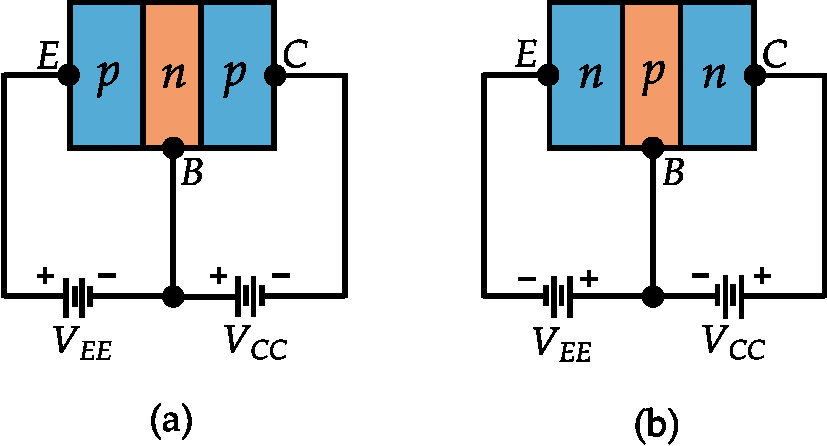
\includegraphics[height=3cm,width=7cm]{diagram-20211104(16)-crop}
	\caption{(a)pnp transistor (b)npn tranasistor}
	\label{}
\end{figure}
Both biasing potentials have been applied to a pnp transistor,large number of majority carriers will diffuse across the forwardbiased p-n junction into the n-type material. The question then is whether these carriers will contribute directly to the base current B or pass directly into the p-type material. Since the sandwiched n-type material is very thin and has a low conductivity, a very small number of these carriers will take this path of high resistance to the base terminal.The magnitude of the
base current is typically on the order of microamperes, as compared to milliamperes for the emitter and collector currents. The larger number of these majority carriers will diffuse across the reverse-biased junction into the p-type material connected to the collector terminal.The reason for the relative ease with which the majority carriers can cross the reverse-biased junction is easily understood if we consider that for the reverse-biased diode the injected majority carriers will appear as minority carriers in the n-type material. In other words, there has been an injection of minority carriers into the n-type base region material.Combining this with the fact that all the minority carriers in the depletion region will cross the
reverse-biased junction of a diode.\\
Applying Kirchhoff's current law to the transistor  as if it were a single node,we obtain
$$I_{E}=I_{}+I_{B}$$
and find that the emitter current is the sum of the collector and base currents.\\
 The collector current, however, comprises two components-the majority and the minority carriers.The minority-current component is called the leakage current and is given the symbol $I_{co}\left(I_{c}\right.$ current with emitter terminal Open). The collector current, therefore, is determined in total by
 $$I_{c}=I_{c_{\text {majoily }}}+I_{co_{\text {minority }}}$$
 For general-purpose transistors, $I_{c}$ is measured in milliamperes and $I_{C O}$ is measured in microamperes or nanoamperes. $I_{co}$, like $I_{s}$ for a reverse-biased diode, is temperature sensitive and must be examined carefully when applications of wide temperature ranges are considered.\\
 \begin{note}
 	\begin{itemize}
 		\item $I_{co}$ for Germanium transisitor is $\mu A$ range, Si transisitor is $nA$ range.\\
 		\item $I_{co}$ doubles for every $10^{\circ}C$ rise in temperature.\\
 		\item For $1^{\circ}C$ ,$I_{co}$  approximately increases by $7\%$
 		$$I_{co(T_2)}=I_{co(T_1)}2^{\left( \frac{T_2-T_1}{10}\right) }$$
 		\item $I_{co}$ is independent of collector supply voltage.\\
 		\item The collector current is less than the emitter current.There are two reason for it.Firstly a part of the emitter current consists of holes that donot contribute to the collector current.secondly not all the  electrons injected in to the base are successful in reaching the collector. 
 	\end{itemize}
 \end{note}
\paragraph{Equation of emitter current}
 In a transistor under active region emitter current is the forward current of emitter diode.\\
 $$I_{E}=I_{co}e^{\frac{V_{BE}}{nV_T}}$$
 The emitter current exponentially increases with base to emitter voltage$V_{BE}$ of the transistor
 \paragraph{Symbol}
 \begin{figure}[H]
 	\centering
 	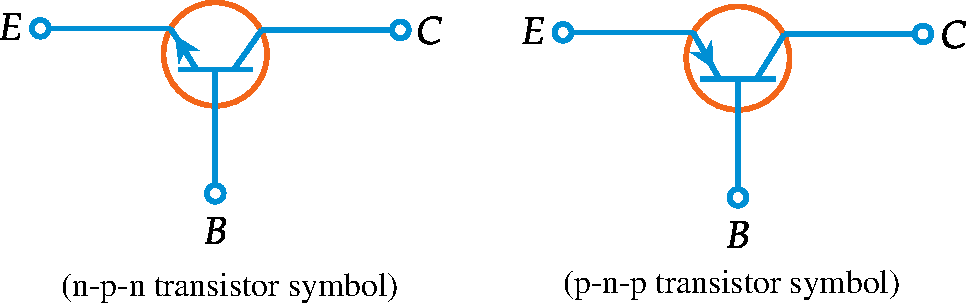
\includegraphics[height=3.5cm,width=11cm]{diagram-20211104(17)-crop}
 	\caption{}
 	\label{}
 \end{figure}
 \paragraph{Modes of operation}
 $$\begin{array}{|c|c|c|c|}
 	\hline \text { Modeof Operations } & \mathrm{J}_{1} \text { (B-E) } & \mathrm{J}_{2} \text { (C-B) } & \text { Applications } \\
 	\hline \text { Active region } & \text { FB } & \text { RB } & \text { As an amplifier } \\
 	\hline \text { Saturation region } & \text { FB } & \text { FB } & \text { As an electronic switch } \\
 	\hline \text { Cut-off region } & \text { RB } & \text { RB } & \text { In digital circuit } \\
 	\hline \begin{array}{l}
 		\text { Reverse active mode or } \\
 		\text { inverted mode }
 	\end{array} & \text { RB } & \text { FB } & \begin{array}{l}
 		\text { As an amplifier with voltage and } \\
 		\text { current gain to below (attenuator) }
 	\end{array} \\
 	\hline
 \end{array}$$
 \section{Transistor configurations}
 There are three leads in a transistor viz., emiter, base and collector terminals. However. when a transistor is to be connected in a circuit, we require four terminals; two for the input and two for the output. This difficulty is overcome by making one terminal of the transistor common to both input and output terminals. The input is fed between this common terminal and one of the other two terminals. The output is obtained between the common terminal and the remaining terminal. Accordingly; a transistor can be connected in a circuit in the following three ways;
 \begin{enumerate}
 	\item Common base configuration
 	\item Common emitter configuration
 	\item Common collector configuration
 \end{enumerate}

 \section{Common base configuration}
 In this circuit arrangement, input is applied between emitter and base and output is taken from collector and base. Here, base of the transistor is common to both input and output circuits.\\
\begin{figure}[H]
	\centering
	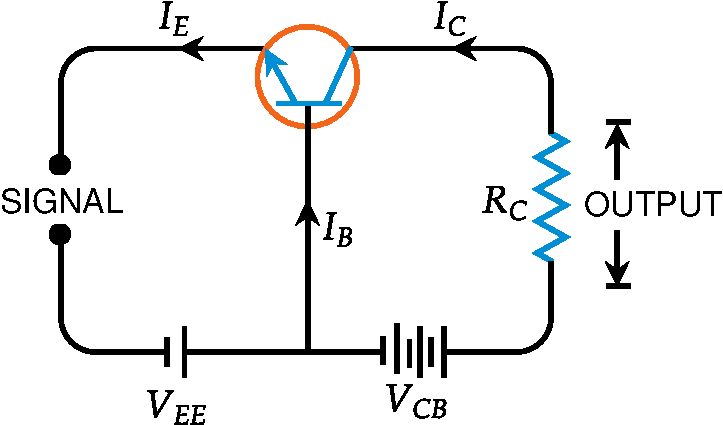
\includegraphics[height=4cm,width=6cm]{diagram-20211105-crop}
	\caption{}
	\label{}
\end{figure}
 To fully describe the behaviour of a three terminal devices such as the common base amplirier,requires two set of characteristics one for the 'driving point' or input parameters and the other forthe output side.
 \subsection{Input characterestics}
 The input set for the common-base amplifier as shown in figure relates an input current $\left(\mathrm{I}_{\mathrm{E}}\right)$ to an input voltage $\left(V_{B E}\right)$ for various levels of output voltage $V_{C B}$.\\
 \begin{figure}[H]
 	\centering
 	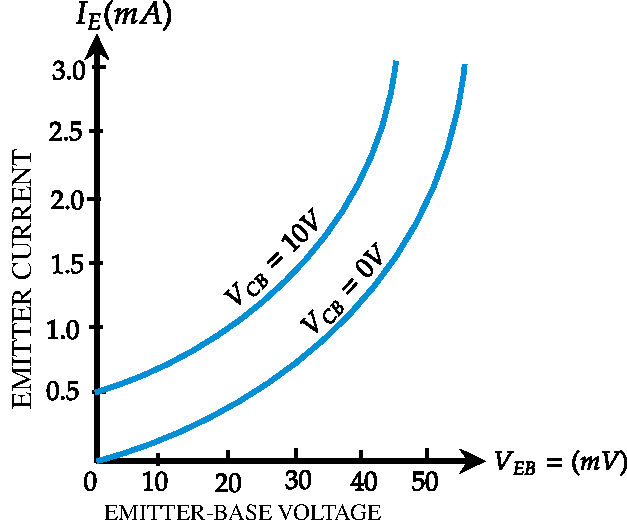
\includegraphics[height=4.5cm,width=6cm]{diagram-20211104(19)-crop}
 	\caption{}
 	\label{}
 \end{figure}
 \textbf{Input resistance.}\\
  It is the ratio of change in emitter-base voltage $\left(\Delta V_{E B}\right)$ to the resulting change in emitter current $\left(\Delta l_{E}\right)$ at constant collector-base voltage $\left(V_{C B}\right)$ i.e.
 Input resistance
  $$r_{i}=\frac{\Delta V_{E B}}{\Delta I_{E}} \text{at constant } V_{C B}$$
 In fact, input resistance is the opposition offered to the signal current. As a very small $V_{E B}$ is sufficient to produce a large flow of emitter current $I_{E}$, therefore, input resistance is quite small, of the order of a few ohms.
 \subsection{output characterestics}
 It relates $I_C$ to $V_{CB}$ for various levels input current $I_E$ shown.\\
\begin{figure}[H]
	\centering
	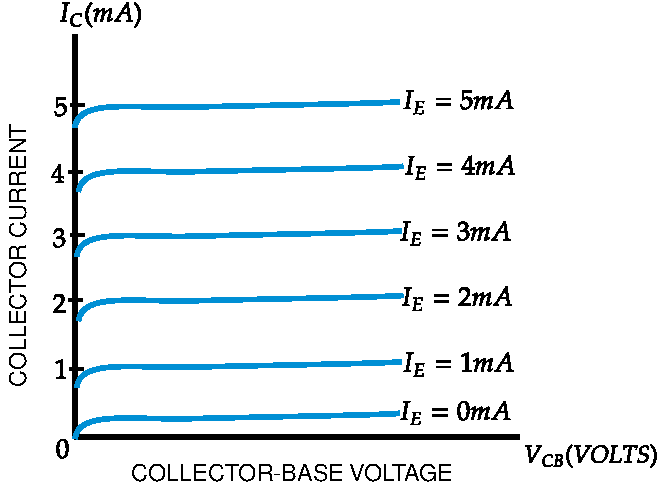
\includegraphics[height=6cm,width=8cm]{diagram-20211104(20)-crop}
	\caption{}
	\label{}
\end{figure}
 From the graph we can say that the emitter current which is approximately equal to collector current.\\
 $$I_{C}\approx I_{E}$$
 \textbf{Output resistance}.\\
  It is the ratio of change in collector-base voltage $\left(\Delta V_{C B}\right)$ to the resulting change in collector current $\left(\Delta I_{C}\right)$ at constant emitter current $i . e$.
 Output resistance,\\
  $$r_{o}=\frac{\Delta V_{C B}}{\Delta I_{C}} \text{ at constant} I_{E}$$
 The output resistance of $C B$ circuit is very high, of the order of several tens of kilo-ohms. This is not surprising because the collector current changes very slightly with the change in $V_{C B}$.
 \subsection{Properties of CB configuration}
 \begin{itemize}
 	\item Lowest input resistance $\left(\mathrm{R}_{\mathrm{i}}<100 \Omega\right)$
 \item	Highest output resistance $\left(\mathrm{R}_{0}>1 \mathrm{M} \Omega\right)$
 \item	Lowest current gain $(\alpha<1)$
 \item	Highest voltage gain
 \item	Medium power gain (typical value 68 )
 \item	Output and input voltages are in phase i.e. phase shift is $0^{\circ}$.
 \item	In $C B$ amplifier current gain is loss and therefore bandwidth is large and hence $C B$ amplifier is widely used as high frequency.\\
 \subsection{Current amplification factor Alpha($\alpha$)}
 \item In the dc mode the levels of $I_{C}$ and $I_{E}$ due to the majority carriers are related by a quantity called alpha and defined by the following equation.
 $$
 \alpha_{d c}=\left|\frac{I_{C}}{I_{E}}\right|
 $$
 Where $I_{C B O}$ is collector to base current when emitter terminal is open.
 \item For ac situations where the point of operation moves on the characteristic curve, an ac alpha is defined by.
 $$\alpha_{ac}=\left.\frac{\Delta I_{C}}{\Delta I_{E}}\right|_{V_{CB-constant}}$$
 \item The alpha is formally called common base amplification factor on current gain of common base transistor.
 \textbf{Note}: The transistor's amplifying action is basically due to its capability of transfer its signal current from a low resistance circuit to high resistance circuit, contracting the two terms transfer and resistor results in the name transistor; i.e\\
  transfer+resistance  $\rightarrow $ transistor 
 \end{itemize}
\subsection{Expression for collector current}
$$\alpha=\frac{I_C}{I_E}$$
$$I_C=\alpha I_E$$ 
The leakage current $I_{leakage}$ is due to the movement of minority carriers across base collector junction on account of it being reverse biased.This is much smaller than $\alpha I_E$
Total collector current\\
$$I_C=\alpha I_E+I_{leakage}$$
It is clear that if $I_E=0$ (emitter circuit is open) a small leakage current still flows in the collector circuit.This leakage is abbreviated as $I_{CBO}$ meaning collector base current with emitter open.Then 
$$I_C=\alpha I_E+I_{CBO}$$
$$I_E=I_C+I_B$$
$$I_C=\alpha(I_C+I_B)+I_{CBO}$$
$$I_C(1-\alpha)=\alpha I_B+I{CBO}$$
$$I_C=\frac{\alpha}{1-\alpha}I_B+\frac{I_{CBO}}{1-\alpha}$$
 \section{Common emitter configuration}
 In this circuit arrangement, input is applied between base and emitter and output is taken from the collector and emitter. Here, emitter of the transistor is common to both input and output circuits and hence the name common emitter connection.\\
 \begin{figure}[H]
 	\centering
 	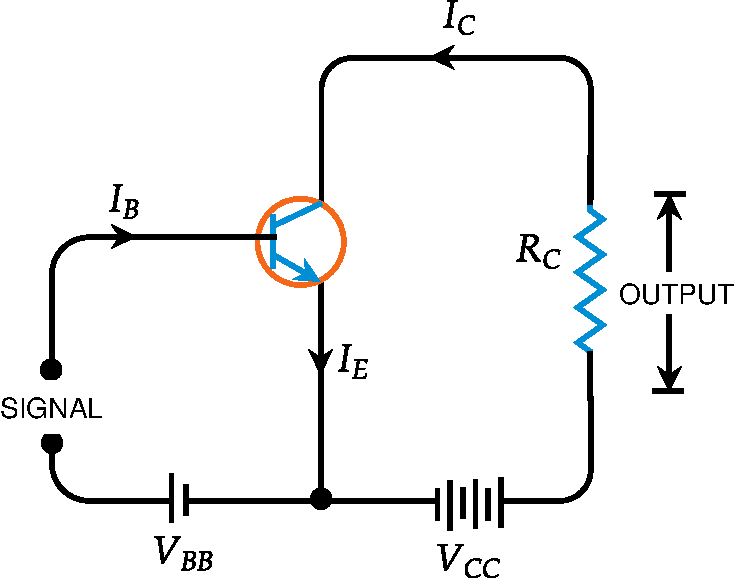
\includegraphics[height=4.5cm,width=6cm]{diagram-20211105(7)-crop}
 	\caption{}
 	\label{}
 \end{figure}
 \subsection{Input characterestics}
  It is the curve between base current $I_{B}$ and base-emitter voltage $V_{B E}$ at constant collector-emitter voltage $V_{C E}$
  \begin{figure}[H]
  	\centering
  	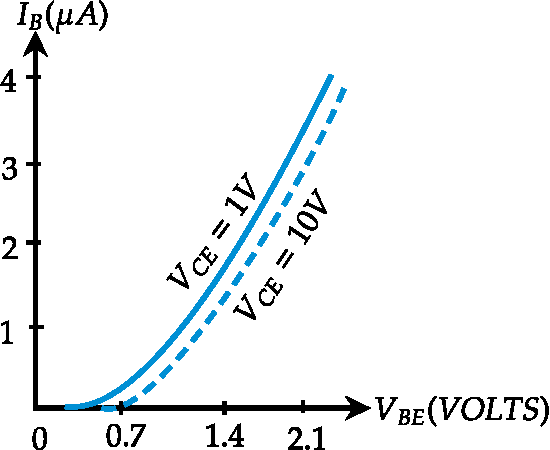
\includegraphics[height=4.5cm,width=6cm]{diagram-20211105(6)-crop}
  	\caption{}
  	\label{}
  \end{figure}
  (i) The characteristic resembles that of a forward biased diode curve. This is expected since the base-emitter section of transistor is a diode and it is forward biased.\\
  (ii) As compared to $C B$ arrangement, $I_{B}$ increases less rapidly with $V_{B E}$. Therefore, input resistance of a $C E$ circuit is higher than that of $C B$ circuit\\
   \textbf{Input resistance.}\\
    It is the ratio of change in base-emitter voltage $\left(\Delta V_{B E}\right)$ to the change in base current $\left(\Delta l_{B}\right)$ at constant $V_{C E}$ i.e.
   Input resistance,
   $$
   r_{i}=\frac{\Delta V_{B E}}{\Delta I_{B}} \text { at constant } V_{C E}
   $$
   The value of input resistance for a $C E$ circuit is of the order of a few hundred ohms.
   \subsection{Output characterestics}
 It is the curve between collector current $I_{C}$ and collector-emitter voltage $V_{C E}$ at constant base current $I_{B}$.\\
 \begin{figure}[H]
 	\centering
 	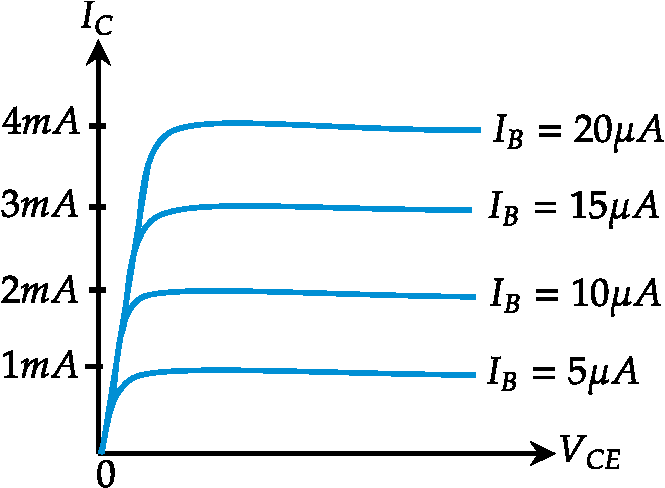
\includegraphics[height=4cm,width=5cm]{diagram-20211105(5)-crop}
 	\caption{}
 	\label{}
 \end{figure}
 The following points may be noted from the characteristics:-\\
 (i) The collector current $I_{C}$ varies with $V_{C E}$ for $V_{C E}$ between 0 and $1 \mathrm{~V}$ only. After this, collector current becomes almost constant and independent of $V_{C E}$. This value of $V_{C E}$ upto which collector current $I_{C}$ changes with $V_{C E}$ is called the knee voltage $\left(V_{\text {knee }}\right)$. The transistors are always operated in the region above knee voltage.\\
 (ii) Above knee voltage, $I_{C}$ is almost constant. However, a small increase in $I_{C}$ with increasing $V_{C E}$ is caused by the collector depletion layer getting wider and capturing a few more majority carriers before electron-hole combinations occur in the base area.\\
 (iii) For any value of $V_{C E}$ above knee voltage, the collector current $I_{C}$ is approximately equal to $\beta \times I_{B}$.\\
  \textbf{Output resistance}
  It is the ratio of change in collector-emitter voltage $\left(\Delta V_{C E}\right)$ to the change in collector current $\left(\Delta I_{C}\right)$ at constant $I_{B}$ i.e.
  Output resistance, $$\quad r_{o}=\frac{\Delta V_{C E}}{\Delta I_{C}}$$ at constant $I_{B}$\\
  \begin{itemize}
  	\item The output resistance of a common emitter configuration is less that of common base configuration.
  \end{itemize}
  \subsection{Current amplification factor Beta ($\beta$)}
  \begin{itemize}
  	\item  For dc $$ \beta_{d c}=\frac{I_{C}}{I_{B}} \quad(\beta>1)$$
  	\item  For ac $$\beta_{a c}=\left.\frac{\Delta I_{C}}{\Delta I_{B}}\right|_{V_{CE=constant}}$$
  	\item Range of $ \beta$ is 30  to 300.
  	\item $\beta$ is called the current gain of transistor in CE mode. It is the most important specification of the transistor.
  	\item $\beta$ is also denoted by $ h_{f e}$
  	\item 
  	$$I_{C}=\beta I_{B}$$
  		$$\mathrm{I}_{\mathrm{E}}=\mathrm{I}_{\mathrm{C}}+\mathrm{I}_{\mathrm{B}}=\beta \mathrm{I}_{\mathrm{B}}+\mathrm{I}_{\mathrm{B}} \quad I_{E}=(\beta+1) I_{B}$$
  		\item Thereia phase difference of $180^{\circ}C$ between input and output voltage  in a CE amplifie.\\
  		 when base voltage increase, base current increases. It causes an increase in collector current also. The collector current causes a voltage drop in the collector resistor. Because the output is situated below the collector resistance (with reference to Vcc) the output voltage will decrease as voltage drop across collector resistor increase. Thus it produces a 180 phase shift. (input positive, output negative and vice versa)
  	\end{itemize}
  		\textbf{Relation between $\alpha$ and $\beta$}\\
  		 $\beta$ in terms of $\alpha$ is $\beta=\frac{\alpha}{1-\alpha}$  $\quad \alpha=\frac{\beta}{1+\beta}$
\subsection{Expression for collector current}
 In common emitter circuit, $I_{B}$ is the input current and $I_{C}$ is the output current.
We know,
$$
I_{E}=I_{B}+I_{C}
$$
and
$$I_{C}=\alpha I_{E}+I_{C B O}$$

From above two equations we will get $$\quad I_{C}=\alpha I_{E}+I_{C B O}=\alpha\left(I_{B}+I_{C}\right)+I_{C B O}$$
or
$$
I_{C}(1-\alpha)=\alpha I_{B}+I_{C B O}
$$
$$
I_{C}=\frac{\alpha}{1-\alpha} I_{B}+\frac{1}{1-\alpha} I_{C B O}
$$
From expression it is apparent that if $I_{B}=0$ (i.e. base circuit is open), the collector current will be the current to the emitter. This is abbreviated as $I_{C E O}$, meaning collector-emitter current with base open.\\
$$I_{CEO}=\frac{1}{1-\alpha}I_{CBO}$$
Then $$I_C=\frac{\alpha}{1-\alpha} I_{B}+I_{CEO}$$
$$I_C=\beta I_B+I_{CEO}$$
\section{Common collector configuration} 
In this circuit arrangement, input is applied between base and collector while the output is taken between the emitter and collector. Here, collector of the transistor is common to both input and the output circuit. Hence the name common collector configuration.
 \subsection{Current amplification factor gamma ($\gamma$)}
 In common collector circuit, input current is the base current $I_{B}$ and output current is the emitter current $I_{E}$. Therefore, current amplification in this circuit arrangement can be defined as under :
 
 The ratio of change in emitter current $\left(\Delta I_{E}\right)$ to the change in base current $\left(\Delta I_{B}\right)$ is known as current amplification factor in common collector (CC) arrangement i.e.
 $$
 \gamma=\frac{\Delta I_{E}}{\Delta I_{B}}
 $$
 This circuit provides about the same current gain as the common emitter circuit as $\Delta I_{E} \simeq \Delta I_{C}$. However, its voltage gain is always less than $1 .$\\
 \textbf{ Relation between$ \gamma$  and $ \alpha$}
 $$
 \begin{aligned}
 \gamma &=\frac{\Delta I_{E}}{\Delta I_{B}} \\
 \alpha &=\frac{\Delta I_{C}}{\Delta I_{E}} \\
 I_{E} &=I_{B}+I_{C} \\
 \Delta I_{E} &=\Delta I_{B}+\Delta I_{C} \\
 \Delta I_{B} &=\Delta I_{E}-\Delta I_{C}
 \end{aligned}
 $$
 Substituting the value of $\Delta I_{B}$ in first expression we get,
 $$
 \gamma=\frac{\Delta I_{E}}{\Delta I_{E}-\Delta I_{C}}
 $$
 Dividing the numerator and denominator on R.H.S. by $\Delta I_{E}$, we get,
 $$
 \begin{aligned}
 &\gamma=\frac{\frac{\Delta I_{E}}{\Delta I_{E}}}{\frac{\Delta I_{E}}{\Delta I_{E}-\frac{\Delta I_{C}}{\Delta I_{E}}}}=\frac{1}{1-\alpha} \quad\left(\because \alpha=\Delta I_{C} / \Delta I_{E}\right) \\
 &\therefore \quad \gamma=\frac{1}{1-\alpha}
 \end{aligned}
 $$
 \subsection{Expression for collector current}
 $$
 \begin{aligned}
 	I_{C} &=\alpha I_{E}+I_{C B O} \\
 	I_{E} &=I_{B}+I_{C}=I_{B}+\left(\alpha I_{E}+I_{C B O}\right) \\
 	I_{E}(1-\alpha) &=I_{B}+I_{C B O} \\
 	I_{E} &=\frac{I_{B}}{1-\alpha}+\frac{I_{C B O}}{I-\alpha} \\
 	I_{E} &=*(\beta+1) I_{B}+(\beta+1) I_{C B O}
 \end{aligned}
 $$
 \subsection{Applications}
  The common collector circuit has very high input resistance (about 750 $\mathrm{K} \Omega$ ) and very low output resistance (about $25 \Omega$ ). Due to this reason, the voltage gain provided by this circuit is always less than 1 . Therefore, this circuit arrangement is seldom used for amplification. However, due to relatively high input resistance and low output resistance, this circuit is primarily used for impedance matching i.e. for driving a low impedance load from a high impedance source.\\
  This configuration is used in emitter follower circuits.
  $$\begin{aligned}
  	&\text { Comparison between CB, CE and CC amplifier }\\
  	&\begin{array}{|l|l|l|l|}
  		\hline \multirow{2}{*}{\text { Characteristic }} & \text { Amplifier } & \multicolumn{2}{l}{} \\
  		\cline { 2 - 4 } & \text { CB } & \text { CE } & \text { CC } \\
  		\hline \text { Input resistance } & \approx 50 \text { to } 200 \Omega & \approx 1 \text { to } & \approx 150-800 \mathrm{k} \Omega \\
  		\left(R_{i}\right) & \text { low } & 2 \mathrm{k} \Omega \text { medium } & \text { high } \\
  		\hline \begin{array}{l}
  			\text { Output resistance } \\
  			\left(R_{o}\right)
  		\end{array} & \begin{array}{l}
  			\approx 1-2 \mathrm{k} \Omega \\
  			\text { high }
  		\end{array} & \begin{array}{l}
  			\approx 50 \mathrm{k} \Omega \\
  			\text { medium }
  		\end{array} & \approx \mathrm{k} \Omega \text { low } \\
  		\hline \text { Current gain } & 0.8-0.9 \text { low } & 20-200 \text { high } & 20-200 \text { high } \\
  		\hline \text { Voltage gain } & \text { Medium } & \text { High } & \text { Low } \\
  		\hline \text { Power gain } & \text { Medium } & \text { High } & \text { Low } \\
  		\hline \begin{array}{l}
  			\text { Phase difference } \\
  			\text { between input and }
  		\end{array} & \text { Zero } & 180^{\circ} & \text { Zero } \\
  		\text { output voltages } & & & \\
  		\hline \begin{array}{l}
  			\text { Used as amplifier } \\
  			\text { for }
  		\end{array} & \text { current } & \text { Power } & \text { Voltage } \\
  		\hline
  	\end{array}
  \end{aligned}$$
 \section{Modes of operation}
 A transistor can be operated in three mode.
 \begin{itemize}
 	\item Saturation region
 	\item Active region
 	\item Cut off region
 	 \end{itemize}
 	\subsection{Load line analysis}
 	\begin{figure}[H]
 		\centering
 		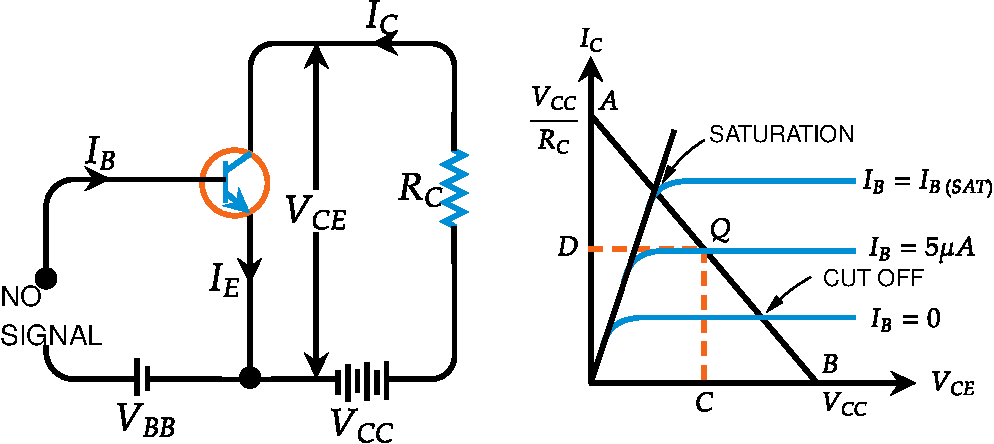
\includegraphics[height=4.5cm,width=10cm]{diagram-20211105(2)-crop}
 		\caption{}
 		\label{}
 	\end{figure}
 	In general we need to determine the the collector current for various collector emitter voltages.One of the method is to plot the output characterestics.But we have another convenient method called load line method wich is used to solve such problems.Consider a circuit as shown in the figure.in this circuit we are not applying any input signal.Only dc conditions prevail in the circuit.\\
 	The value of collector emitter voltage at any time is given by\\
 	$$V_{CE}=V_{CC}-I_CR_C$$
 	In this equation $V_{CC}$ and $R_C$ are constants.if we plot $I_C$ against $V_{CE}$(Same as the case of output characterestics) we will get a straight line with end pointts as $\frac{V_CC}{R_C}$ at A on $I_C$ axis and $V_{CC}$ at B on $V_{CE}$ axis.\\This line $AB$ is called load line.\\
 	The load line meet at some point on the output characterestics is called quiscent point or $Q-$point.\\
 	The corresponding value of $I_c$ and $V_{CE}$ ie(C,D) is called operating point.\\
 	It is called operating point because the variation of $I_C$ and $V_{CE}$ take place about this point when signal is applied.
\subsection{Modes}
(i)$\textbf{Cut off }$
The point where th load line intersects the "$I_B=0$" curve is known as \textit{cut off}.\\
At this point $I_B=0$ and only small collector current(ie the collector leakage $I_{CEO} $ exists.\\
At cut off the base emitter junction no longer forward biased and normal transistor action is lost.\\
The collector emitter voltage is nearly equal to $V_{CC}$\\
(ii)\textbf{Saturation}\\
The points where the load line intersects the $I_B=I_B{(sat)}$ curve is called saturation\\
$I_B=I_B{{sat}}$ curve means it is the maximum base current when the collector base junction is not reverse biased.\\
At this point the transisitor will not work.\\
At this point $I_C $ is approximately equal to $\frac{V_{CC}}{R_C}$\\
(iii)\textbf{Active region}
The region between cut off and saturation is known as active region.\\
In the active region collector base junction remains reverse biased while base emitter junction remains forward biased.\\
Consequently the transisitor will function normally in this region.\\
\textbf{CUT-OFF }: Emitter diode and collector diode are OFF.\\
\textbf{ACTIVE }: Emitter diode is ON and collector diode is OFF.\\
\textbf{SATURATED }: Emitter diode and collector diode are ON.
\section{Power rating of a transisitor}
\textit{The maximum power that a transistor can handle without destruction is known as power rating of the transistor.}
When a transistor is in operation, almost all the power is dissipated at the reverse biased collector-base junction.\\
 The power rating (or maximum power dissipation) is given by:
$$P_{D(\max )} =\text { Collector current } \times \text { Collector-base voltage }$$
$$=I_{C} \times V_{C B}$$
$$\therefore \quad P_{D(\max )} =I_{C} \times V_{C E} \\
\left[\because V_{C E}=V_{C B}+V_{B E} \cdot \text { Since } V_{B E} \text { is very small, } V_{C B} \simeq V_{C E}\right]
$$
While connecting transistor in a circuit, it should be ensured that its power rating is not exceeded otherwise the transistor may be destroyed due to excessive heat.
\section{Transisitor biasing}
   For faithfull amplification a transisitor amplifier must satisfy three basic conditions.namely\\
   (i)Proper zero signal collector current\\
   {(ii)}Proper base emitter voltage at any instant.\\
   (iii)Proper collector emitter voltage at any instant.\\
The proper zerosignal collector current means that the applied signal that should be amplified must not cut off at any portion of the signal.Zero signal current must be greater than the maximum value of collector current due to signal alone.\\
   The other two conidtions is to keep the base emitter junction properly forward biased and collector base junction properly reverse biased during the application of the signal.\\
   All these conditions are fullfilled by transisitor biasing.
   \subsection{Methods of transister biasing}
   In the transistor amplifier circuits drawn so far biasing was done with the aid of a battery $V_{B B}$ which was separate from the battery $V_{C C}$ used in the output circuit. However, in the interest of simplicity and economy, it is desirable that transistor circuit should have a single source of supply-the one in the output circuit (i.e. $V_{C C}$ ). The following are the most commonly used methods of obtaining transistor biasing from one source of supply (i.e. $V_{C C}$ ):\\
   (i) Base resistor method\\
   (ii) Biasing with collector-feedback resistor\\
   (iii) Voltage-divider bias
   \subsection{Base resistor method}
   \begin{figure}[H]
   	\centering
   	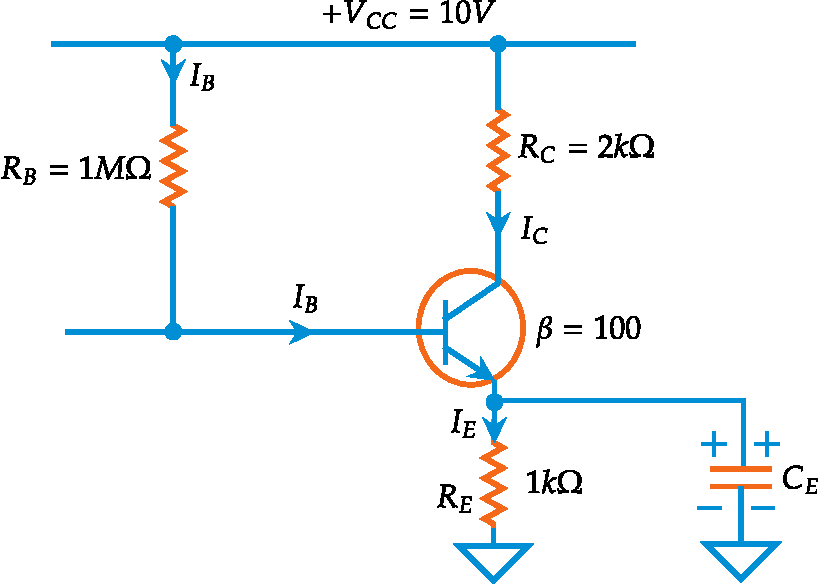
\includegraphics[height=5cm,width=7cm]{diagram-20211108(16)-crop}
   	\caption{}
   	\label{}
   \end{figure}
   In this method, a high resistance $R_{B}$ (several hundred $\mathrm{k} \Omega$ ) is connected between the base and +ve end of supply for $n p n$. transistor  and between base and negative end of supply for $p n p$ transistor.\\
   The required value of $R_B$  that can be found out as \\
   $$
   I_{B}=\frac{I_{C}}{\beta}
   $$
   Considering the closed circuit $A B E N A$ and applying Kirchhoff's voltage law, we get,
   $$
   \begin{aligned}
   & V_{C C} &=I_{B} R_{B}+V_{B E} \\
   \text { or } & I_{B} R_{B} &=V_{C C}-V_{B E} \\
   & \therefore \quad R_{B} &=\frac{V_{C C}-V_{B E}}{I_{B}}
   \end{aligned}
   $$
   $V_{BE}$ is small compared to $V_{CC}$  we can neglect it.Then\\
   $$R_B=\frac{V_{CC}}{I_B}$$
   Since the base bias current $I_B$ is constant,the circuit is called fixed bias circuit.Applying KVL around the collector emitter circuit we get
   $$V_{CC}=I_CR_C+V_{CE}$$
   \paragraph{Stability factor}
   Stability factor, $$\quad S=\frac{\beta+1}{1-\beta\left(\frac{d I_{B}}{d I_{C}}\right)}$$
   In fixed-bias method of biasing, $I_{B}$ is independent of $I_{C}$ so that $d I_{B} / d I_{C}=0$.\\
    Putting the value of $d I_{B} / d I_{C}=0$ in the above expression, we have,
   $$\text{ Stability factor }S=\beta+1$$
   This method provides poor stabilisation. It is because there is no means to stop a self-increase in collector current due to temperature rise and individual variations.The stability factor is very high. Therefore, there are strong chances of thermal runaway.\\
   Due to these disadvantages, this method of biasing is rarely employed.
   \begin{exercise}
   {(i)}	A germanium transistor is to be operated at zero signal $I_C=1mA$ .If the collector supply $V_{CC}=12V$. what is the value of $R_B$ in the base resisitor method ?Take $\beta=100$\\
   {(ii)} If another transisitor of the same batch with $\beta=50$ is used.What will be the new value zero signal $I_C$ for the same $R_B$
   \end{exercise}
\begin{answer}(i)
	$$R_B=\frac{V_{CC}-V_{BE}}{I_B}$$
	$$V_{BE}=0.3V \quad V_{CC}=12V \quad I_B=\frac{I_C}{\beta}$$
	$$I_B=\frac{1mA}{100}=0.01mA$$
	$$R_B=\frac{12-0.3}{0.01mA}=\frac{11.7}{0.01mA}=1170K\Omega$$
	(ii)
	$\beta=50$\\
	$$V_{CC}=I_BR_B+V_{BE}$$
	$$I_B=\frac{V_{CC}-V_{BE}}{R_B}=\frac{12-0.3}{1170K\Omega}=0.01mA$$
	$$I_C=\beta I_B=50\times 0.01=0.5mA$$
\end{answer}
\begin{exercise}
	Calculate the values of three currents in the circuit shown in Figure?
	\begin{figure}[H]
		\centering
		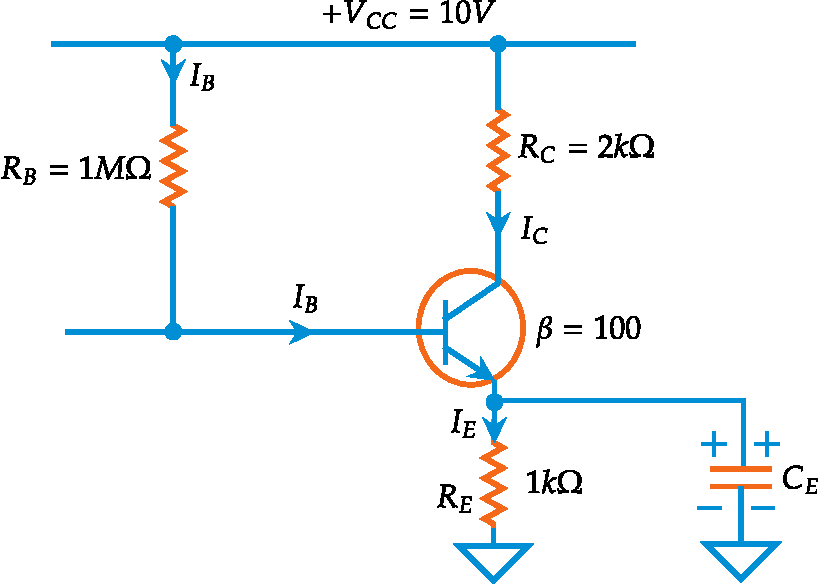
\includegraphics[height=5cm,width=7cm]{diagram-20211108(16)-crop}
		\caption{}
		\label{}
	\end{figure}
\end{exercise}
\begin{answer} Applying Kirchhoff 's voltage law to the base side and taking resistances in $\mathrm{k} \Omega$ and currents in $\mathrm{mA}$, we have,	
	$$\begin{aligned}
		V_{C C} &=I_{B} R_{B}+V_{B E}+I_{E} \times 1k\Omega\\
		\text{we can neglect $V_{BE}$ which is small}\\
		10 &=1000k\Omega I_{B}+ 0+\left(I_{C}+I_{B}\right) \\
		10 &=1000 I_{B}+\left(\beta I_{B}+I_{B}\right) \\
		10 &=1000 I_{B}+\left(100 I_{B}+I_{B}\right) \\
		10 &=1101 I_{B}k\Omega \\
		I_{B} &=10 / 1101=0.0091 \mathrm{~mA} \\
		I_{C} &=\beta I_{B}=100 \times 0.0091=0.91 \mathrm{~mA} \\
		I_{E} &=I_{C}+I_{B}=0.91+0.0091=0.919 \mathrm{~mA}
	\end{aligned}$$
\end{answer}
   \subsection{Biasing with feedback resistor}
   \begin{figure}[H]
   	\centering
   	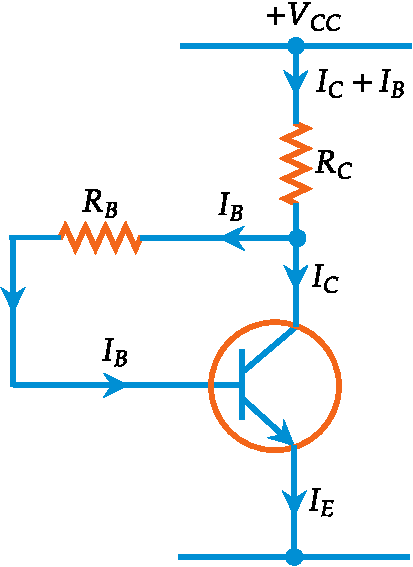
\includegraphics[height=6cm,width=5cm]{diagram-20211109-crop}
   	\caption{}
   	\label{}
   \end{figure}
   In this method, one end of $R_{B}$ is connected to the base and the other end to the collector as shown in Figure. Here, the required zero signal base current is determined not by $V_{C C}$ but by the collector base voltage $V_{CB}$.\\
   The required value of $R_{B}$ needed to give the zero signal current $I_{C}$ can be determined as follows.
   $$
   \begin{aligned}
   V_{C C} &=* I_{C} R_{C}+I_{B} R_{B}+V_{B E} \\
   R_{B} &=\frac{V_{C C}-V_{B E}-I_{C} R_{C}}{I_{B}} \\
   &=\frac{V_{C C}-V_{B E}-\beta I_{B} R_{C}}{I_{B}} \quad\left(\because I_{C}=\beta I_{B}\right)
   \end{aligned}
   $$
   Alternatively, $V_{C E}=V_{B E}+V_{C B}$
   or
   $$
   \begin{aligned}
   &\text { or } \quad V_{C B}=V_{C E}-V_{B E} \\
   &\therefore \quad R_{B}=\frac{V_{C B}}{I_{B}}=\frac{V_{C E}-V_{B E}}{I_{B}} ; \quad \text { where } \quad I_{B}=\frac{I_{C}}{\beta}
   \end{aligned}
   $$
   \paragraph{Stability factor}
   Stability factor, $S<(\beta+1)$\\
   Therefore, this method provides better thermal stability than the fixed bias.
   \paragraph{Operating points $I_C$ and $V_{CE}$}
   $$\begin{aligned}
   	I_{C} &=\frac{V_{C C}-V_{B E}}{R_{B} / \beta+R_{C}} \\
   	V_{C E} &=V_{C C}-I_{C} R_{C}
   \end{aligned}$$
   \paragraph{Disadvantages}
    The circuit does not provide good stabilisation because stability factor is fairly high.Therefore, the operating point does change, although to lesser extent, due to temperature variations and other effects.\\
    This circuit provides a negative feedback which reduces the gain of the amplifier.
    \subsection{Voltage divider bias method}
   \begin{figure}[H]
   	\centering
   	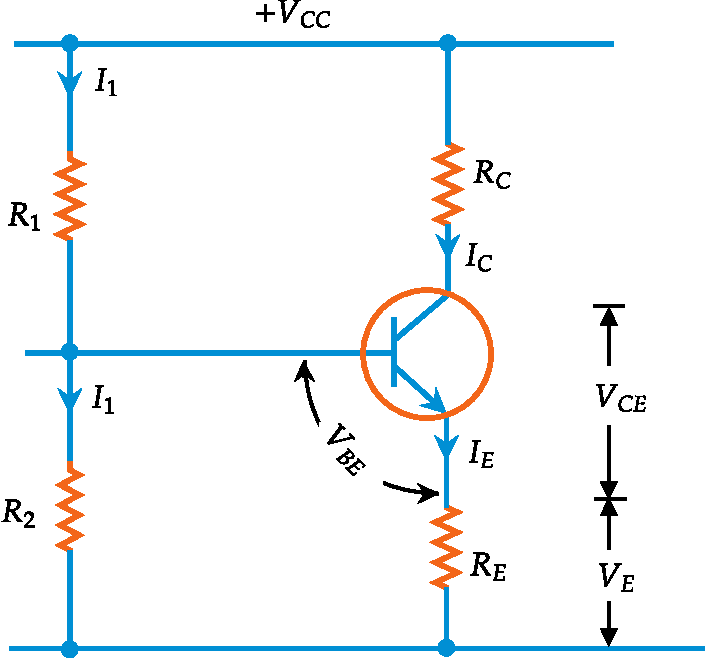
\includegraphics[height=5.5cm,width=6cm]{diagram-20211109(8)-crop}
   	\caption{}
   	\label{}
   \end{figure}
    This is the most widely used method of providing biasing and stabilisation to a transistor. In this method, two resistances $R_{1}$ and $R_{2}$ are connected across the supply voltage $V_{C C}$ and provide biasing. The emitter resistance $R_{E}$ provides stabilisation. The name "voltage divider" comes from the voltage divider formed by $R_{1}$ and $R_{2}$. The voltage drop across $R_{2}$ forward biases the base-emitter junction. This causes the base current and hence collector current flow in the zero signal conditions.\\
     Suppose that the current flowing through resistance $R_{1}$ is $I_{1} .$ As base current $I_{B}$ is very small, therefore, it can be assumed with reasonable accuracy that current flowing through $R_{2}$ is also $I_{1}$.\\
    (i) \textbf{Collector current} $\mathrm{I}_{\mathrm{C}}$ :
    $$
    I_{1}=\frac{V_{C C}}{R_{1}+R_{2}}
    $$
    $\therefore \quad$ Voltage across resistance $R_{2}$ is
    $$
    V_{2}=\left(\frac{V_{C C}}{R_{1}+R_{2}}\right) R_{2}
    $$
    Applying Kirchhoff's voltage law to the base circuit of Fig. $9.24$,
    or
    $$
    \begin{aligned}
    &V_{2}=V_{B E}+V_{E} \\
    &V_{2}=V_{B E}+I_{E} R_{E}
    \end{aligned}
    $$
    or $\quad$ Since $I_{E} \simeq I_{C}$ 
    $$\therefore I_{C}=\frac{V_{2}-V_{B E}}{R_{E}}$$
   It is clear from the above expression that $I_{C}$ does not at all depend upon $\beta$. Though $I_{C}$ depends upon $V_{B E}$ but in practice $V_{2}>>V_{B E}$ so that $I_{C}$ is practically independent of $V_{B E}$. Thus $I_{C}$ in this circuit is almost independent of transistor parameters and hence good stabilisation is ensured. It is due to this reason that potential divider bias has become universal method for providing transistor biasing.\\
   (ii) \textbf{Collector-emitter voltage} $\mathbf{V}_{\mathrm{CE}}$.\\
    Applying Kirchhoff's voltage law to the collector side,
   $$
   V_{C C}=I_{C} R_{C}+V_{C E}+I_{E} R_{E}
   $$
   $$
   \begin{aligned}
   	&=I_{C} R_{C}+V_{C E}+I_{C} R_{E} \\
   	&=I_{C}\left(R_{C}+R_{E}\right)+V_{C E} \\
   	V_{C E} &=V_{C C}-I_{C}\left(R_{C}+R_{E}\right)
   \end{aligned}
   $$
   \paragraph{Stabilisation.}
    In this circuit, excellent stabilisation is provided by $R_{E}\\
    $ Consideration the equation
   $$
   V_{2}=V_{B E}+I_{C} R_{E}
   $$
   Suppose the collector current $I_{C}$ increases due to rise in temperature. This will cause the voltage drop across emitter resistance $R_{E}$ to increase. As voltage drop across $R_{2}\left(\right.$ i.e. $\left.V_{2}\right)$ is independent of $I_{C}$, therefore, $V_{B E}$ decreases. This in turn causes $I_{B}$ to decrease. The reduced value of $I_{B}$ tends to restore $I_{C}$ to the original value.
   \paragraph{Stability factor}
    $$\text{ Stability factor } =(\beta+1) \times \frac{1}{\beta+1}=1$$This is the smallest possible value of S and leads to the maximum possible thermal stability.\\
    \paragraph{Operating points}
    We know that$$V_{C E} =V_{C C}-I_{C}\left(R_{C}+R_{E}\right)$$
    $$\text{ when } I_C=0 \quad  V_{CE}=V_{CC}$$
    $$\text{and when } V_{CE}=0 \quad I_{C}=\frac{V_{CC}}{R_C+R_E}$$
    \begin{note}
    	Voltage drop across $R_2$\\
    	$$V_2=\frac{V_{CC}}{R_1+R_2}.R_2$$
    	And effective base resistance $$R_B=\frac{R_1R_2}{R_1+R_2}$$
    	Application of KVL around the base circuit yields,\\
    	$$V=I_BR_B+V_{BE}+I_ER_E$$	
    \end{note}
\begin{exercise}
	 A transistor uses potential divider method of biasing. $R_{1}=50 \mathrm{k} \Omega, R_{2}=10 \mathrm{k} \Omega$ and $R_{E}=1 \mathrm{k} \Omega$. If $V_{C C}=12 \mathrm{~V}$, find :\\
(i) the value of $I_{C}$; given $V_{B E}=0.1 \mathrm{~V}$\\
(ii) the value of $I_{C} ;$ given $V_{B E}=0.3 \mathrm{~V}$. 	
\end{exercise}
\begin{answer}
$R_{1}=50 \mathrm{k} \Omega, R_{2}=10 \mathrm{k} \Omega, R_{E}=1 \mathrm{k} \Omega, V_{C C}=12 \mathrm{~V}$\\
(i) When $V_{B E}=0.1 \mathrm{~V}$,\\
Voltage across $R_{2}$ $$V_{2}=\frac{R_{2}}{R_{1}+R_{2}} V_{C C}=\frac{10}{50+10} \times 12=2 \mathrm{~V}$$
$$V_2=V_{BE}+I_ER_E \quad I_E\approx I_C$$
$$\therefore \quad
 Collector current, I_{C}=\frac{V_{2}-V_{B E}}{R_{E}}=\frac{2-0.1}{1 \mathrm{k} \Omega}=1.9 \mathrm{~mA}$$
 (ii) When $V_{B E}=0.3 \mathrm{~V}$,
 Collector current, $$I_{C}=\frac{V_{2}-V_{B E}}{R_{E}}=\frac{2-0.3}{1 \mathrm{k} \Omega}=1.7 \mathrm{~mA}$$	
\end{answer}

\section{Transisitor amplifiers}
A transistor raises the strength of a weak signal and thus acts as an amplifier. The weak signal is applied between emitter-base junction and output is taken across the $\log R_{C}$ connected in the collector circuit. \\
As the input circuit has low resistance, therefore, a small change in signal voltage causes an appreciable change in emitter current. This causes almost the same change in collector current due to transistor action. The collector current flowing through a high load resistance $R_{C}$ produces a large voltage across it. Thus, a weak signal applied in the input circuit appears in the amplified form in the collector circuit. It is in this way that a transistor acts as an amplifier.
\subsection{Single stage transistor amplifier}
When only one transistor with associated circuitry is used for amplifying a weak signal, the circuit is known as single stage transistor amplifier.\\
\textbf{Cicuit analysis}\\
\begin{figure}[H]
	\centering
	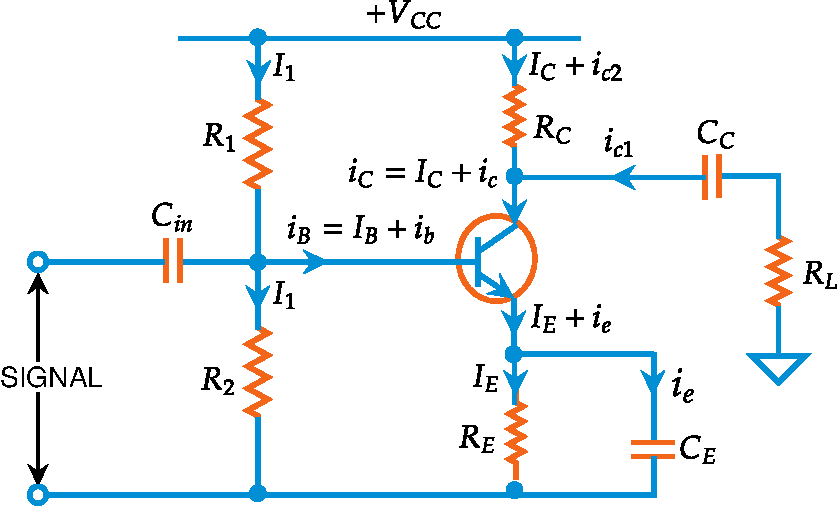
\includegraphics[height=6cm,width=9cm]{diagram-20211108(15)-crop}
	\caption{}
	\label{}
\end{figure}
(i)\textbf{Biasing circuit}\\
The resistances $R_{1}, R_{2}$ and $R_{E}$ form the biasing and stabilisation circuit. The biasing circuit must establish a proper operating point otherwise a part of the negative half-cycle of the signal may be cut off in the output.\\
(ii)\textbf{Input capacitor $C_{in}$}\\
An electrolytic capacitor $C_{i n}(\simeq 10 \mu \mathrm{F})$ is used to couple the signal to the base of the transistor. If it is not used, the signal source resistance will come across $R_{2}$ and thus change the bias. The capacitor $C_{i n}$ allows only a.c. signal to flow but isolates the signal source from $R_{2} *$\\
(iii)\textbf{Emitter bypass capacitor $C_E$}\\
An emitter bypass capacitor $C_{E}(\simeq 100 \mu F)$ is used in parallel with $R_{E}$ to provide a low reactance path to the amplified a.c. signal. If it is not used, then amplified a.c. signal flowing through $R_{E}$ will cause a voltage drop across it, thereby reducing the output voltage.\\
(iv)\textbf{Coupling capacitor $C_C$}
The coupling capacitor $C_{C}(\simeq 10 \mu F)$  couples one stage of amplification to the next stage. If it is not used, the bias conditions of the next stage will be drastically changed due to the shunting effect of $R_{C} .$ This is because $R_{C}$ will come in parallel with the upper resistance $R_{1}$ of the biasing network of the next stage, thereby altering the biasing conditions of the latter. In short, the coupling capacitor $C_{C}$ isolates the d.c. of one stage from the next stage, but allows the passage of a.c. signal.\\
(ii)\textbf{Phase reversal}
In common emitter connection, when the input signal voltage increases in the positive sense, the output voltage increases in the negative direction and vice-versa. In other words, there is a phase difference of $180^{\circ}$ between the input and output voltage in $C E$ connection. This is called phase reversal.*

The phase difference of $180^{\circ}$ between the signal voltage and output voltage in a common emitter amplifier is known as phase reversal.\\
(iii)\textbf{Voltage gain}\\
\begin{figure}[H]
	\centering
	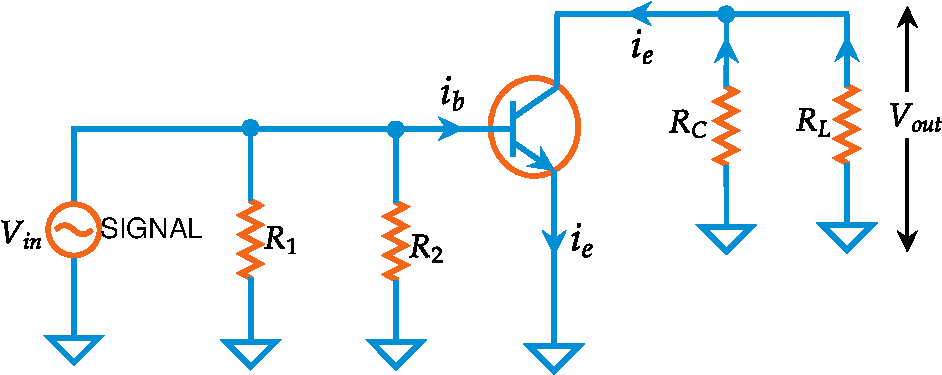
\includegraphics[height=4cm,width=9cm]{diagram-20211108(14)-crop}
	\caption{}
	\label{}
\end{figure}
\par The basic function of an amplifier is to raise the strength of an a.c. input signal. The voltage gain of the amplifier is the ratio of a.c. output voltage to the a.c. input signal voltage. Therefore, in order to find the voltage gain, we should consider only the a.c. currents and voltages in the circuit. For this purpose, we should look at the a.c. equivalent circuit of transistor amplifier.\\
It is clear that as far as a.c. signal is concerned, load $R_{C}$ appears in parallel with $R_{L}$.\\ Therefore, effective load for a.c. is given by:\\
a.c. load, $$R_{A C}=R_{C} \| R_{L}=\frac{R_{C} \times R_{L}}{R_{C}+R_{L}}$$
Output voltage, $$V_{\text {out }}=i_{c} R_{A C}$$
Input voltage, $$V_{i n}=i_{b} R_{i n}$$
$\therefore \quad$ Voltage gain, $A_{v}=V_{o u l} / V_{\dot{m} n}$
$$
=\frac{i_{c} R_{A C}}{i_{b} R_{i n}}=\beta \times \frac{R_{A C}}{R_{i n}} \quad\left(\mathrm{Q} \frac{i_{c}}{i_{b}}=\beta\right)
$$
Incidentally, power gain is given by;
$$
A_{p}=\frac{i_{c}^{2} R_{A C}}{i_{b}^{2} R_{i n}}=\beta^{2} \times \frac{R_{A C}}{R_{i n}}
$$
(iv)\textbf{Gian and transisitor configurations}
\par We know that the process of raising the strength of an a.c. signal is called amplification and the circuit used to preform this function is called an amplifier. There are three types of gain : current gain, voltage gain and power gain.\\
(i) The common emitter (CE) amplifier exhibits all there types gain. From input to output, current will increase, voltage will increase and power will increase.\\
(ii) The common base (CB) amplifier has voltage gain and power gain but no current gain. Note that the current gain of a $C B$ circuit is less than 1 .\\
(iii) The common collector $(C C)$ amplifier has current gain and power gain but no voltage gain.
\begin{exercise}
	 In a transistor amplifier, when the signal changes by $0.02 \mathrm{~V}$, the base current changes by $10 \mu \mathrm{A}$ and collector current by $1 \mathrm{~mA}$. If collector load $R_{C}=5 \mathrm{k} \Omega$ and $R_{L}=10 \mathrm{k} \Omega$, find: (i) current gain (ii) input impedance (iii) a.c. load (iv) voltage gain (v) power gain.
\end{exercise}
\begin{answer}
 $\quad \Delta I_{B}=10 \mu \mathrm{A}, \Delta I_{C}=1 \mathrm{~mA}, \Delta V_{B E}=0.02 \mathrm{~V}, R_{C}=5 \mathrm{k} \Omega, R_{L}=10 \mathrm{k} \Omega$\\
	(i) $\quad$ Current gain, $\beta=\frac{\Delta I_{C}}{\Delta I_{B}}=\frac{1 m A}{10 \mu A}=\mathbf{1 0 0}$\\\\
	(ii) $\quad$ Input impedance, $R_{i n}=\frac{\Delta V_{B E}}{\Delta I_{B}}=\frac{0.02 V}{10 \mu A}=2 \mathrm{k} \Omega$\\\\
	(iii) $\quad$ a.c. load, $R_{A C}=\frac{R_{C} \times R_{L}}{R_{C}+R_{L}}=\frac{5 \times 10}{5+10}=3.3 \mathrm{k} \Omega$\\\\
	(iv) Voltage gain, $A_{v}=\beta \times \frac{R_{A C}}{R_{i n}}=100 \times \frac{3.3}{2}=165$\\\\
	(v) $\quad$ Power gain, $A_{p}=$ current gain $\times$ voltage gain $=100 \times 165=16500$
\end{answer}
\subsection{classificaton of transistor amplifiers}
\par The transistor amplifiers may be classified as to their usage, frequency capabilities, coupling methods and mode of operation.
\begin{enumerate}
	\item \textbf{According to use:}\\
	The classifications of am-plifiers as to usage are basically voltage amplifiers and
	power amplifiers.
	\item \textbf{According to frequency capabilities:}\\
	According to frequency capabilities, amplifiers are clas-sified as audio amplifiers, radio frequency amplifiers.
	\item \textbf{According to coupling methods:}\\
	The output from a single stage amplifier is usually insuf-
	ficient to meet the practical requirements. Additional amplification is often necessary. To do this, the output of one stage is coupled to the next stage. Depending upon the coupling device used, the amplifiers are classified as R-C coupled amplifiers, transformer coupled amplifiers etc.
	\item \textbf{According to mode of operation:}\\
	The amplifiers are frequently classified according to their mode of operation as class A, class B and class C amplifiers.
\end{enumerate}


\subsection{Multi stage transistor amplifier}
\textit{A transistor circuit containing more than one stage of amplification is known as multistage transistor amplifier.}
In a multistage amplifier, a number of single amplifiers are connected in cascade arrangement i.e. output of first stage is connected to the input of the second stage through a suitable coupling device and so on. The purpose of coupling device $(e . g .$ a capacitor, transformer etc. $)$ is,
\begin{itemize}
	\item   To transfer a.c. output of one stage to the input of the next stage.
	\item   To isolate the d.c. conditions of one stage from the next stage.
\end{itemize}
There are mainly three type of coupling present.
\begin{enumerate}
	\item \textbf{RC coupling}\\
	A capacitor is used as the coupling device. The capacitor connects the output of one stage to the input of the next stage in order to pass the a.c. signal on while blocking the d.c. bias voltages
	\item  \textbf{In transformer coupling,} \\
	transformer is used as the coupling device. The transformer coupling provides the same two functions (viz. to pass the signal on and blocking d.c.) but permits in addition impedance matching.
	\item \textbf{In direct coupling or d.c. coupling.}
	
\end{enumerate}
The individual amplifier stage bias conditions are so designed that the two stages may be directly connected without the necessity for d.c. isolation.

 
 \paragraph{Important terms}
 \begin{enumerate}
 	\item \textbf{Gain}\\
  The ratio of the output electrical quantity to the input one of the amplifier is called its gain.
  The gain of a multistage amplifier is equal to the product of gains of individual stages. For instance, if $G_{1}, G_{2}$ and $G_{3}$ are the individual voltage gains of a three-stage amplifier, then total voltage gain $\mathrm{G}$ is given by :
  $$
  G=G_{1} \times G_{2} \times G_{3}
  $$
  \item \textbf{Frequency response}	\\
  The voltage gain of an amplifier varies with signal frequency. It is because the reactance of the capacitors in the circuit changes with signal frequency and hence affects the output voltage. The curve between voltage gain and signal
  frequency of an amplifier is known as frequency re-
  sponse. The gain of the amplifier increases as the frequency increases from zero till it becomes maximum at $f_r$ , called resonant frequency. If the frequency of signal increases beyond $f_r$ , the gain decreases.\\
  \begin{figure}[H]
  	\centering
  	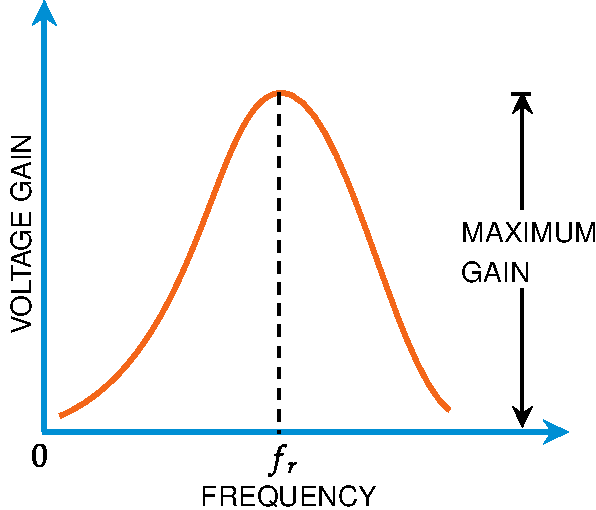
\includegraphics[height=4cm,width=5cm]{diagram-20211108-crop}
  	\caption{}
  	\label{}
  \end{figure}
 \item  \textbf{Decibel gain}\\
 The unit assigned for gain is bel or decibel (db).
 The common logarithm (log to the base 10) of power gain is known as bel power gain i.e.
 $$
 \begin{aligned}
 \text { Power gain } &=\log _{10} \frac{P_{\text {out }}}{P_{\text {in }}} \text { bel } \\
 1 \text { bel } &=10 \mathrm{db}
 \end{aligned}
 $$
 $$
 \therefore \quad \text { Power gain }=10 \log _{10} \frac{P_{o u t}}{P_{i n}} d b
 $$
 If the two powers are developed in the same resistance or equal resistances, then,
 $$
 \begin{aligned}
 P_{1} &=\frac{V_{i n}^{2}}{R}=I_{i n}^{2} R \\
 P_{2} &=\frac{V_{\text {out }}^{2}}{R}=I_{\text {out }}^{2} R \\
 \therefore \quad \text { Voltage gain in } d b &=10 \log _{10} \frac{V_{\text {out }}^{2} / R}{V_{\text {in }}^{2} / R}=20 \log _{10} \frac{V_{\text {out }}}{V_{\text {in }}} \\
 \text { Current gain in } d b &=10 \log _{10} \frac{I_{\text {out }}^{2} R}{I_{\text {in }}^{2} R}=20 \log _{10} \frac{I_{\text {out }}}{I_{\text {in }}}
 \end{aligned}
 $$
 \item \textbf{Bandwidth.}
 The range of frequency over which the voltage gain is equal to or greater than
 $70.7\%$ of the maximum gain is known as bandwidth.\\
In the figure $f_2-f_1$ is called bandwidth.\\
  The former $\left(f_{1}\right)$ is called lower cut-off frequency and the latter $\left(f_{2}\right)$ is known as upper cut-off frequency. 
  \begin{minipage}{0.5\textwidth}
  	The bandwidth of an amplifier can also be defined in terms of $d b$. Suppose the maximum voltage gain of an amplifier is 100 . Then $70.7 \%$ of it is $70.7$.
  	$\therefore \quad$ Fall in voltage gain from maximum gain
  	$$
  	\begin{aligned}
  	&=20 \log _{10} 100-20 \log _{10} 70.7 \\
  	&=20 \log _{10} \frac{100}{70.7} d b \\
  	&=20 \log _{10} 1.4142 d b=3 d b
  	\end{aligned}
  	$$
  \end{minipage}
  \begin{minipage}{0.5\textwidth}
  	 \begin{figure}[H]
  		\centering
  		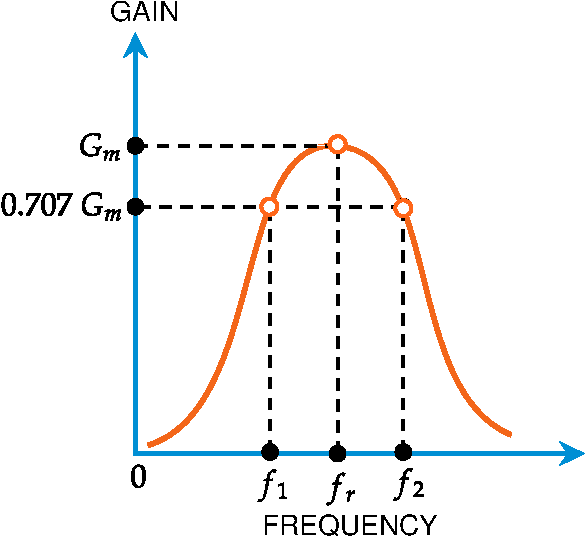
\includegraphics[height=5.5cm,width=6cm]{diagram-20211108(1)-crop}
  		\caption{}
  		\label{}
  	\end{figure}
  \end{minipage}
  Hence bandwidth of an amplifier is the range of frequency at the limits of which its voltage gain falls by 3 db from the maximum gain.\\
  The frequency $f_{1}$ or $f_{2}$ is also called 3-db frequency or half-power frequency.\\
  The $3-d b$ designation comes from the fact that voltage gain at these frequencies is $3 d b$ below the maximum value. The term half-power is used because when voltage is down to $0.707$ of its maximum value, the power (proportional to $V^{2}$ ) is down to $(0.707)^{2}$ or one-half of its maximum value.
 \end{enumerate}
 \begin{exercise}
  A three-stage amplifier has a first stage voltage gain of 100 , second stage voltage gain of 200 and third stage voltage gain of 400 . Find the total voltage gain in $d b$.
 \end{exercise}
\begin{answer}
	\begin{align*}
\text{First-stage voltage gain in} \ d b&=20 \log _{10} 100=20 \times 2=40\\
\text{Second-stage voltage gain in} \ d b&=20 \log _{10} 200=20 \times 2.3=46\\
\text{Third-stage voltage gain in}\ d b&=20 \log _{10} 400=20 \times 2.6=52\\
\text{Total voltage gain}\ &=40+46+52=138 \mathrm{db}
	\end{align*}
	
\end{answer}
\begin{exercise}
 A certain amplifier has voltage gain of $15 \mathrm{db}$. If the input signal voltage is $0.8 \mathrm{~V}$, what is the output voltage?
\end{exercise}
\begin{answer}
	 $$ d b \text { voltage gain } =20 \log _{10} V_{2} / V_{1}$$ 
	 $$15 =20 \log _{10} V_{2} / V_{1}$$ 
	 $$15 =20 \log _{10} V_{2} / 0.8V$$ 
	 $$V_2=10^{\frac{3}{4}}\times 0.8V$$
	 $$V_2=4.5V$$
\end{answer}
\subsection{RC Coupled Transistor Amplifier}
This is the most popular type of coupling because it is cheap and provides excellent audio fidelity over a wide range of frequency. It is usually employed for voltage amplification. Figure shows two stages of an $R C$ coupled amplifier. A coupling capacitor $C_{C}$ is used to connect the output of first stage to the base (i.e. input) of the second stage and so on. As the coupling from one stage to next is achieved by a coupling capacitor followed by a connection to a shunt resistor, therefore, such amplifiers are called resistance - capacitance coupled amplifiers.\\
\begin{figure}[H]
	\centering
	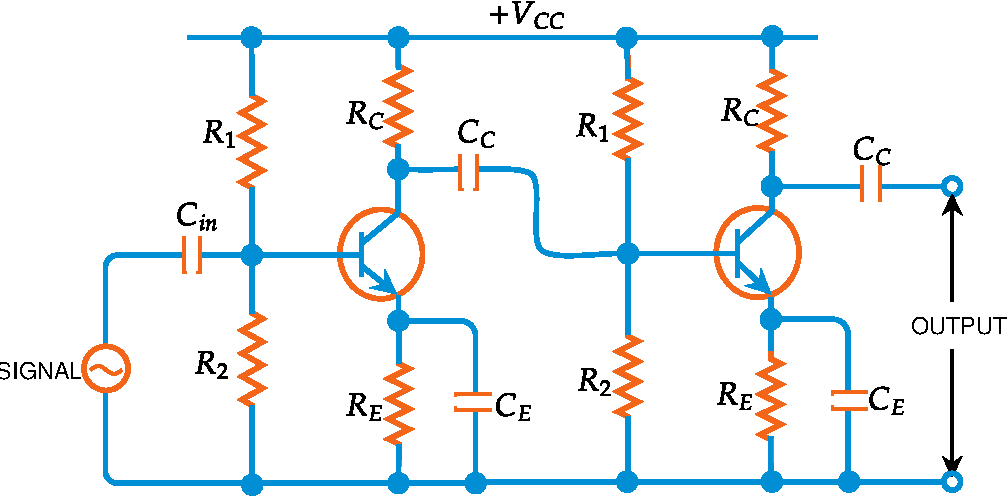
\includegraphics[height=5cm,width=10cm]{diagram-20211108(3)-crop}
	\caption{}
	\label{}
\end{figure}
The resistances $R_{1}, R_{2}$ and $R_{E}$ form the biasing and stabilisation network. The emitter bypass capacitor offers low reactance path to the signal. Without it, the voltage gain of each stage would be lost. The coupling capacitor $C_{C}$ transmits a.c. signal but blocks d.c. This prevents d.c. interference between various stages and the shifting of operating point.\\
\subsubsection{Operation}
 When a.c. signal is applied to the base of the first transistor, it appears in the amplified form across its collector load $R_{C} .$ The amplified signal developed across $R_{C}$ is given to base of next stage through coupling capacitor $C_{C} .$ The second stage does further amplification of the signal. In this way, the cascaded (one after another) stages amplify the signal and the overall gain is considerably increased.

It may be mentioned here that total gain is less than the product of the gains of individual stages. It is because when a second stage is made to follow the first stage, the effective load resistance of first stage is reduced due to the shunting effect of the input resistance of second stage. This reduces the gain of the first stage.

\subsubsection{Frequency response.} 
The frequency response of a typical RC coupled amplifier.
\begin{enumerate}
	\item \textbf{ At low frequencies $(<50 \mathrm{~Hz})$} the reactance of coupling capacitor $C_{C}$ is quite high and hence very small part of signal will pass from one stage to the next stage. Moreover, $C_{E}$ cannot shunt the emitter resistance $R_{E}$ effectively because of its large reactance at low frequencies. These two factors cause a falling of voltage gain at low frequencies.
	\item \textbf{ Athigh frequencies $(>20 \mathrm{kHz})$}The reactance of $C_{C}$ is very small and it behaves as a short circuit. This increases the loading effect of next stage and serves to reduce the voltage gain. Moreover, at high frequency, capacitive reactance of base-emitter junction is low which increases the base current. This reduces the current amplification factor $\beta$. Due to these two reasons, the voltage gain drops off at high frequency.
	\item \textbf{ At mid-frequencies ( $50 \mathrm{~Hz}$ to $20 \mathrm{kHz}$ )}, the voltage gain of the amplifier is constant. The effect of coupling capacitor in this frequency range is such so as to maintain a uniform voltage gain. Thus, as the frequency increases in this range, reactance of $C_{C}$ decreases which tends to increase the gain. However, at the same time, lower reactance means higher loading of first stage and hence lower gain. These two factors almost cancel each other, resulting in a uniform gain at mid-frequency.
\end{enumerate}

\subsubsection{Advantages}
\begin{enumerate}
	\item  It has excellent frequency response. The gain is constant over the audio frequency range which is the region of most importance for speech, music etc.
	\item It has lower cost since it employs resistors and capacitors which are cheap.
	\item The circuit is very compact as the modern resistors and capacitors are small and extremely light.
\end{enumerate}

\subsubsection{Disadvantages}
\begin{enumerate}
	\item The $R C$ coupled amplifiers have low voltage and power gain. It is because the low resistance presented by the input of each stage to the preceding stage decreases the effective load resistance $\left(R_{A C}\right)$ and hence the gain.
	\item They have the tendency to become noisy with age, particularly in moist climates.
	\item Impedance matching is poor. It is because the output impedance of $R C$ coupled amplifier isseveral hundred ohms whereas the input impedance of a speaker is only a few ohms. Hence, little power will be transferred to the speaker.
\end{enumerate}

\section{Transistor oscillators}
\paragraph{Sinusoidal Oscillator}
An electronic device that generates sinusoidal oscillations of desired frequency is known as a sinusoidal oscillator.\\
A transistor amplifier with proper positive feedback can act as an oscillator $i . e .$, it can generate oscillations without any external signal source.A positive feedback amplifier is one that produces a feedback voltage ($V_F$ ) that is in phase with the original input signal.\\
A phase shift of 180° is produced by the amplifier and a further phase shift of 180° is introduced by feedback network. Consequently,the signal is shifted by 360° and fed to the input i.e., feedback voltage is in phase with the input signal.\\
\begin{figure}[H]
	\centering
	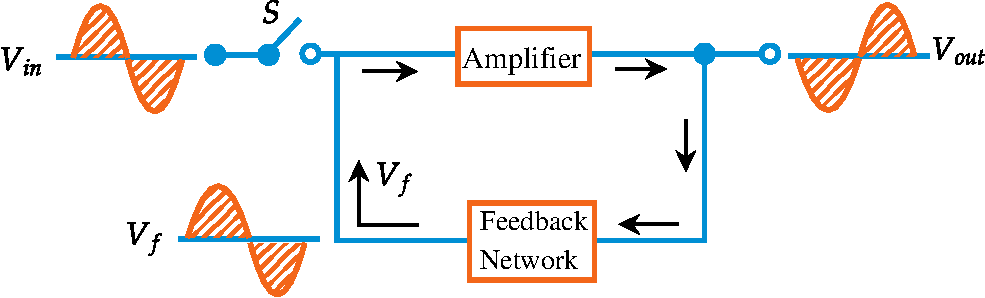
\includegraphics[height=4cm,width=10cm]{diagram-20211106(21)-crop}
	\caption{}
	\label{}
\end{figure}
\par  When we open the switch $S$  the input signal $\left(V_{i n}\right)$ is removed. However, $V_{f}$ (which is in phase with the original signal) is still applied to the input signal. The amplifier will respond to this signal in the same way that it did to $V_{\text {in }}$ i.e., $V_{f}$ will be amplified and sent to the output. The feedback network sends a portion of the output back to the input. Therefore, the amplifier receives another input cycle and another output cycle is produced. This process will continue so long as the amplifier is turned on. Therefore, the amplifer will produce sinusoidal output with no external signal source.
\par  The circuit needs only a quick trigger signal to start the oscillations. Once the oscillations have started, no external signal source is needed.
In order to get continuous undamped output from the circuit, the following condition must be met :
$$
\begin{aligned}
m_{v} A_{v} &=1 \\
A_{v} &=\text { voltage gain of amplifer without feedback } \\
m_{v} &=\text { feedback fraction }
\end{aligned}
$$
This relation is called \textbf{Barkhausen criterion. }\\
\textbf{Explanation.}
 The voltage gain of a positive feedback amplifier is given by;
$$
A_{v f}=\frac{A_{v}}{1-m_{v} A_{v}}
$$
If $m_{v} A_{v}=1$, then $A_{v f} \rightarrow \infty$.
We know that we cannot achieve infinite gain in an amplifier. It means that a vanishing small input voltage would give rise to finite (i.e., a definite amount of) output voltage even when the input signal is zero. Thus once the circuit receives the input trigger, it would become an oscillator, generating oscillations with no external signal source.
\subsection{Essentials of a transistor oscilltor}
\begin{figure}[H]
	\centering
	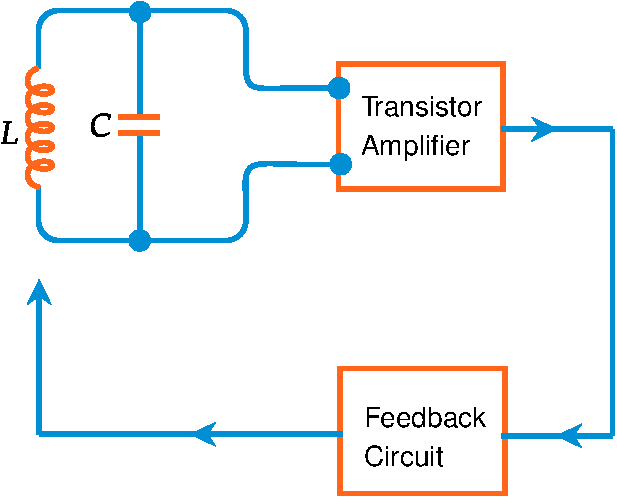
\includegraphics[height=4.5cm,width=6.5cm]{diagram-20211106(22)-crop}
	\caption{}
	\label{}
\end{figure}
\begin{enumerate}
	\item \textbf{Tank circuit}\\
	It consists of inductance coil (L) connected in parallel with capacitor (C). The
	frequency of oscillations in the circuit depends upon the values of inductance of the coil and capaci-tance of the capacitor.
	\item \textbf{Transistor amplifier}
	The transistor amplifier receives d.c. power from the battery and changes it into a.c. power for supplying to the tank circuit. The oscillations occurring in the tank circuit are applied to the input of the transistor amplifier. Because of the amplifying properties of the transistor, we get increased output of these oscillations.
	\item \textbf{Feedback circuit.}
	The feedback circuit supplies a part of collector energy to the tank circuit in correct phase to aid the oscillations i.e. it provides positive feedback.
\end{enumerate}

 \subsection{Different Types of Transistor Oscillators}
 The major difference between these oscillators lies in the method by which energy is supplied to the tank circuit to meet the losses. The following are the transistor oscillators commonly used at various places in electronic circuits:
 \begin{enumerate}
 	\item Tuned collector oscillator
 	\item Colpitt's oscillator
 	\item Hartley oscillator
 	\item Phase shift oscillator
 	\item Wien Bridge oscillator
 	\item Crystal oscillator
 	
 \end{enumerate}

 \subsection{Tuned collector oscillator}
\begin{figure}[H]
	\centering
	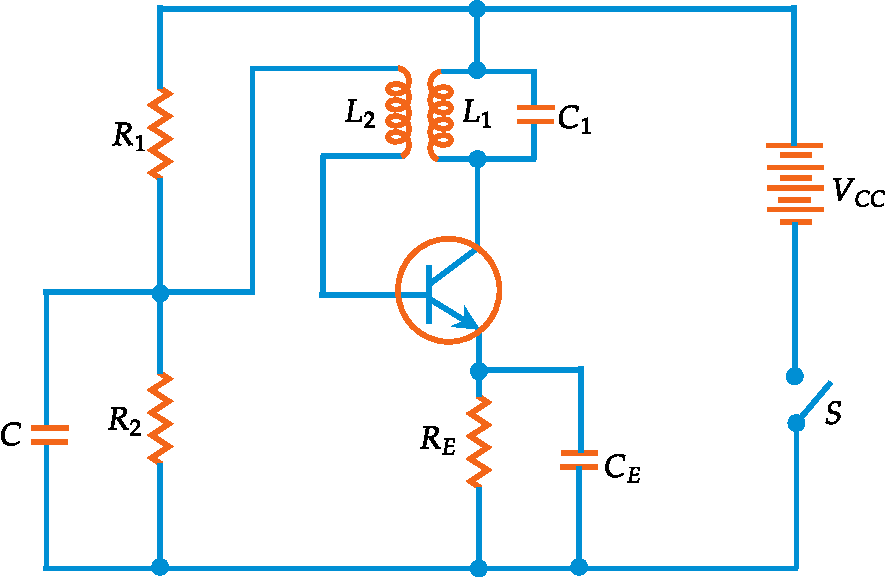
\includegraphics[height=4.7cm,width=8.5cm]{ diagram-20211108(4)-crop}
	\caption{}
	\label{}
\end{figure}
 Figure shows the circuit of tuned collector oscillator. It contains tuned circuit $L_{1}-C_{1}$ in the collector and hence the name. The frequency of oscillations depends upon the values of $L_{1}$ and $C_{1}$ and is given by:
 $$
 f=\frac{1}{2 \pi \sqrt{L_{1} C_{1}}}
 $$
 The feedback coil $L_{2}$ in the base circuit is magnetically coupled to the tank circuit coil $L_{1}$. In practice, $L_{1}$ and $L_{2}$ form the primary and secondary of the transformer respectively. The biasing is provided by potential divider arrangement. The capacitor $C$ connected in the base circuit provides low reactance path to the oscillations.
 \subsection{Colpitt’s Oscillator}
 \begin{figure}[H]
 	\centering
 	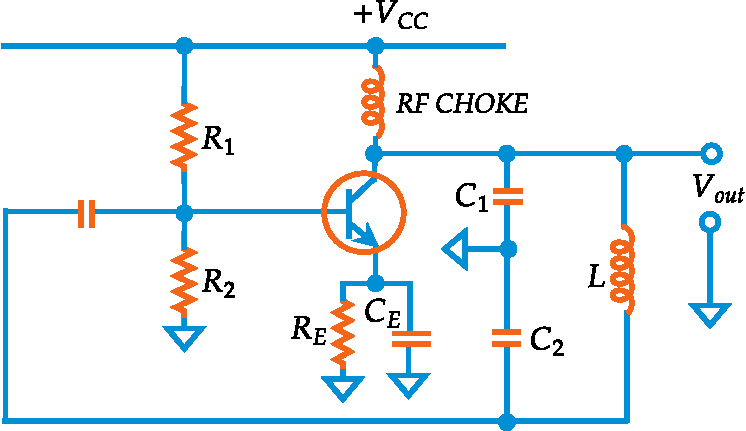
\includegraphics[height=4.8cm,width=8.5cm]{diagram-20211108(6)-crop}
 	\caption{}
 	\label{}
 \end{figure}
 Figure shows a Colpitt's oscillator. It uses two capacitors and placed across a common inductor $L$ and the centre of the two capacitors is tapped. The tank circuit is made up of $C_{1}, C_{2}$ and $L$. The frequency of oscillations is determined by the values of $C_{1}, C_{2}$ and $L$ and is given by ;
 $$
 f=\frac{1}{2 \pi \sqrt{L C_{T}}}
 $$
 $$C_{T}=\frac{C_{1} C_{2}}{C_{1}+C_{2}}$$
 Note that $C_1-C_2-L$ is also the feedback circuit that produces a phase shift of 180°.
 \subsection{Hartley Oscillator}
 \begin{figure}[H]
 	\centering
 	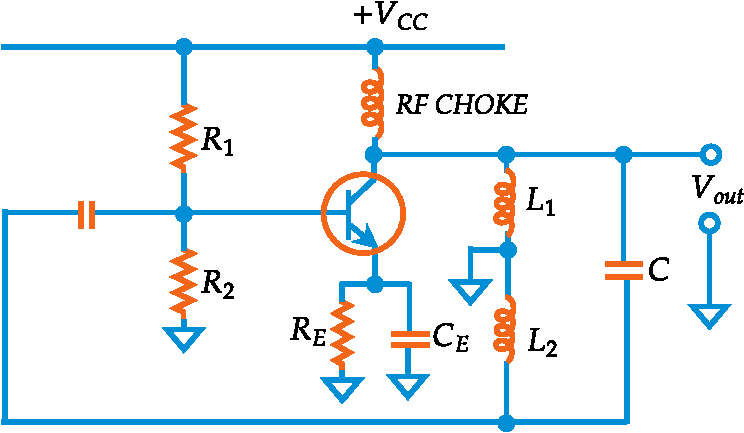
\includegraphics[height=4.5cm,width=8.5cm]{diagram-20211108(7)-crop}
 	\caption{}
 	\label{}
 \end{figure}
 The Hartley oscillator is similar to Colpitt's oscillator with minor modifications. Instead of using tapped capacitors, two inductors $L_{1}$ and $L_{2}$ are placed across a common capacitor $C$ and the centre of the inductors is tapped as shown in Figure. The tank circuit is made up of $L_{1}, L_{2}$ and $C$. The frequency of oscillations is determined by the values of $L_{1}, L_{2}$ and $C$ and is given by :
 where
 $$
 \begin{aligned}
 f &=\frac{1}{2 \pi \sqrt{C L_{T}}} \\
 L_{T} &=L_{1}+L_{2}+2 M \\
 M &=\text { mutual inductance between } L_{1} \text { and } L_{2}
 \end{aligned}
 $$
 Note that $L_{1}-L_{2}-C$ is also the feedback network that produces a phase shift of $180^{\circ}$.
 \subsection{Phase Shift Oscillator}
 \begin{figure}[H]
 	\centering
 	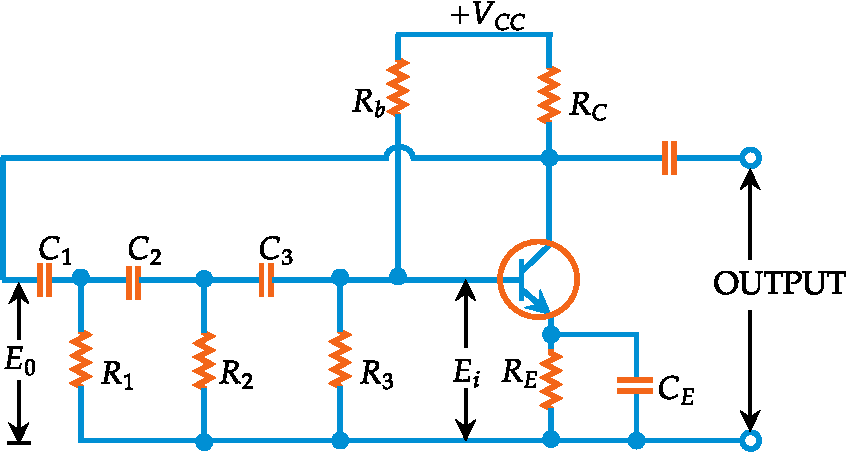
\includegraphics[height=4.5cm,width=8.5cm]{diagram-20211108(5)-crop}
 	\caption{}
 	\label{}
 \end{figure}
 Figure shows the circuit of a phase shift oscillator. It consists of a conventional single transistor amplifier and a $R C$ phase shift network. The phase shift network consists of three sections $R_{1} C_{1}, R_{2} C_{2}$ and $R_{3} C_{3} .$ At some particular frequency $f_{0}$, the phase shift in each $R C$ section is $60^{\circ}$ so that the total phase-shift produced by the $R C$ network is $180^{\circ} .$ The frequency of oscillations is given by:
 $$\begin{aligned}
 	f_{0} &=\frac{1}{2 \pi R C \sqrt{6}} \\
 	R_{1} &=R_{2}=R_{3}=R \\
 	C_{1} &=C_{2}=C_{3}=C
 \end{aligned}$$
 \subsection{Wien Bridge Oscillator}
The Wien-bridge oscillator is the standard oscillator circuit for all frequencies in the range of $10 \mathrm{~Hz}$ to about $1 \mathrm{MHz}$. It is the most frequently used type of audio oscillator as the output is free from circuit fluctuations and ambient temperature. Figure shows the circuit of Wien bridge
 oscillator. It is essentially a two-stage amplifier with $R$ - $C$ bridge circuit.\\
  \begin{figure}[H]
  	\centering
  	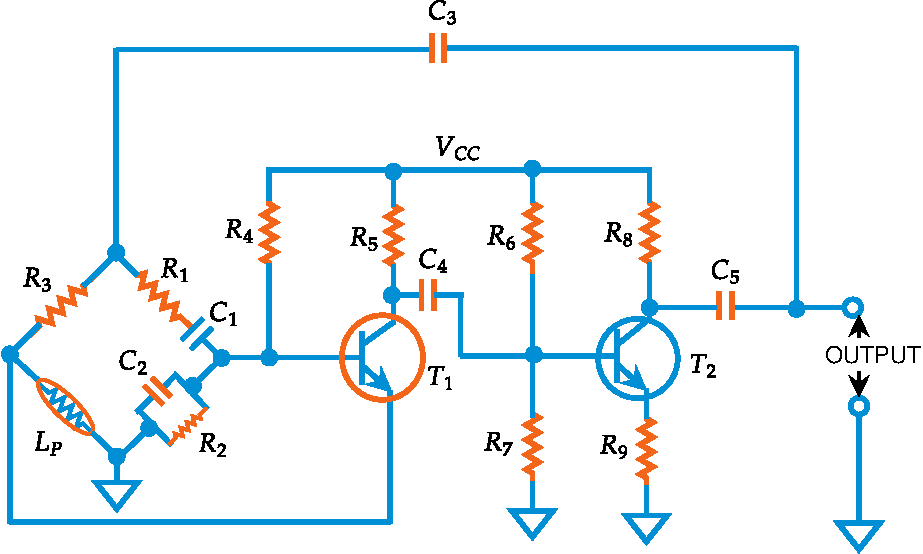
\includegraphics[height=6cm,width=11cm]{diagram-20211108(8)-crop}
  	\caption{}
  	\label{}
  \end{figure}
 \par The bridge circuit has the arms $R_{1} C_{1}$, $R_{3}, R_{2} C_{2}$ and tungsten lamp $L_{p} .$ Resistances $R_{3}$ and $L_{p}$ are used to stabilise the amplitude of the output. The transistor $T_{1}$ serves as an oscillator and amplifier while the other transistor $T_{2}$ serves as an inverter (i.e. to produce a phase shift of $180^{\circ}$ ). The circuit uses positive and negative feedbacks. The positive feedback is through $R_{1} C_{1}, C_{2} R_{2}$ to the transistor $T_{1}$. The negative feedback is through the voltage divider to the input of transistor $T_{2}$. The frequency of oscillations is determined by the series element $R_{1} C_{1}$ and parallel element $R_{2} C_{2}$ of the bridge.
$$
f=\frac{1}{2 \pi \sqrt{R_{1} C_{1} R_{2} C_{2}}}
$$
If $R_{1}=R_{2}=R$
and $C_{1}=C_{2}=C$, then,
$$
f=\frac{1}{2 \pi R C}
$$
\textbf{Advantages}
\begin{itemize}
	\item it gives costant output due to using temperature sensitive tungston lamp $L_p$
	\item The overall gain is high because of two transistors.
	\item The frequency of oscillation can be easily changed by a potentiometer.
	\item The circuit work quite easily.
\end{itemize}
	\textbf{Disadvantages}
\begin{itemize}	
	\item It cannot generate very high frequency.
	\item The circuit requires two transistors and a number of component
\end{itemize}
\subsection{Limitations of L-C and R-C}
\begin{itemize}
	\item Due to some limitations of $L-C$ and $RC$ oscillators ,we need crystal oscillators.
	\item $LC$ oscillators are not used at low frequencies because inductor become bulky and costly.
	\item $RC$ oscillators have not constant frequency and $Q$ factor because of temperature variations.
\end{itemize}
\subsection{Crystal oscillator}
\begin{itemize}
	\item Electrical oscillator cicuits are replaced by mechanical variations circuit that is called crystal oscillator.
	\item Certain crystalline materials ,namely ,roschelle salt,quartz and fourmaline exhibit the piezoelectric effect.
	\item Of the various piezoelectric crystals,quartz is most commonly used because it is inexpensive and their great mechanical strength.\\
		\item When the circuit is not vibrating, it is equivalent to capacitance $\mathrm{C}_{\text {in }}$ because it has two metal plates separated by a dielectric.
	\item When a crystal vibrates, it is equivalent R-L-C series circuit.
	\item Therefore, the equivalent circuit of a vibrating crystal is R-L-C series circuit shunted by the mounting capacitance $C_{m}$ as shown in figure 
	\item Q factor of crystal $Q=\frac{1}{R} \sqrt{\frac{L}{C}}$
	\item Q factor of crystal is very high
\item The extremely high $\mathrm{Q}$ of a crystal leads to frequency stability.
\end{itemize}
\subsubsection{Frequency response of crystal:}
\begin{itemize}
	\item \textbf{Case-I:} When $X_{C}=X_{L}$ at series resonant\\\\
	Impedance of the crystal is very low $\mathrm{Z}=\mathrm{R}$\\
	Series resonant frequency $f_{S}=\frac{1}{2 \pi \sqrt{L C}} H z$\\
	\item \textbf{Case-II:} At a slightly higher frequency, the net reactance of branch $R-L-C$ inductive and equal to $X_{\mathrm{cm}}$
	$$
	X_{L}-X_{c m}
	$$
	The crystal now acts as a parallel resonant circuit Impedance of crystal is very high\\
	Parallel resonant frequency\\
	$$f_{P}=\frac{1}{2 \pi \sqrt{L C_{e q}}}$$ where, $$C_{e q}=\frac{C \times C_{m}}{C+C_{m}}, C_{e q}<C$$
\end{itemize}
\textbf{Advantages:}\\
- It has a high order of frequency stability.\\
- The quality factor $(Q)$ of the crystal is very high. \\\\
\textbf{Disadvantages:}\\
- Hardly tunned\\
- It is fragile and consequently can only be used in low power circuit.
\begin{note}
 At $f_{S}$, the crystal will acts as a series resonant circuit.\\
At $f_{P}$, the crystal will acts as a parallel resonant circuit. 
\end{note}
\newpage
\begin{abox}
	Practise Set-1
	\end{abox}
\begin{enumerate}
	\item The transistor in the given circuit has $h_{f e}=35 \Omega$ and $h_{i e}=1000 \Omega$. If the load resistance $R_{L}=1000 \Omega$, the voltage and current gain are, respectively.
	{	\exyear{NET/JRF(JUNE-2012)}}
	\begin{tasks}(1)
		\task[\textbf{A.}] $-35$ and $+35$
		\task[\textbf{B.}] 35 and $-35$
		\task[\textbf{C.}] 35 and $-0.97$
		\task[\textbf{D.}]  $0.98$ and - 35
	\end{tasks}
	\begin{figure}[H]
		\centering
		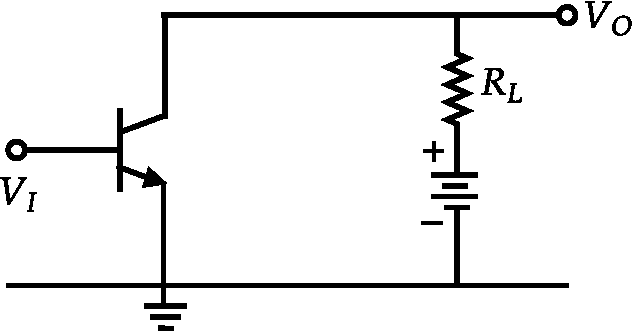
\includegraphics[height=3cm,width=5cm]{e-10}
	\end{figure}
	\item A silicon transistor with built-in voltage $0.7 \mathrm{~V}$ is used in the circuit shown, with $V_{B B}=9.7 V, R_{B}=300 k \Omega, V_{C C}=12 V$ and $R_{C}=2 k \Omega$. Which of the following figures correctly represents the load line and quiescent $Q$ point?
	{	\exyear{NET/JRF(JUNE-2013)}}
	\begin{figure}[H]
		\centering
		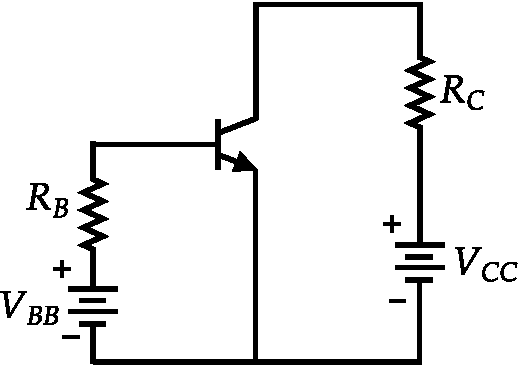
\includegraphics[height=3.5cm,width=5cm]{e-17}
	\end{figure}
	\begin{tasks}(2)
		\task[\textbf{A.}] \begin{figure}[H]
			\centering
			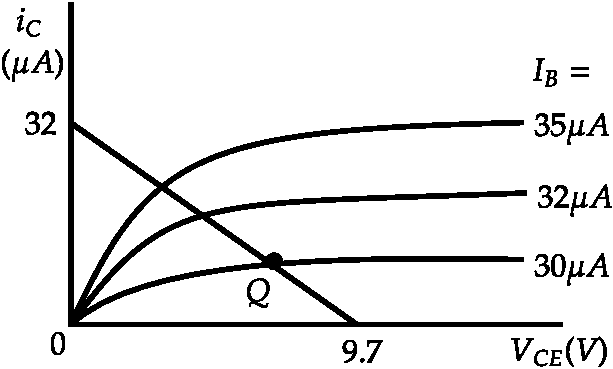
\includegraphics[height=3.3cm,width=5.5cm]{e-17a}
		\end{figure}
		\task[\textbf{B.}] \begin{figure}[H]
			\centering
			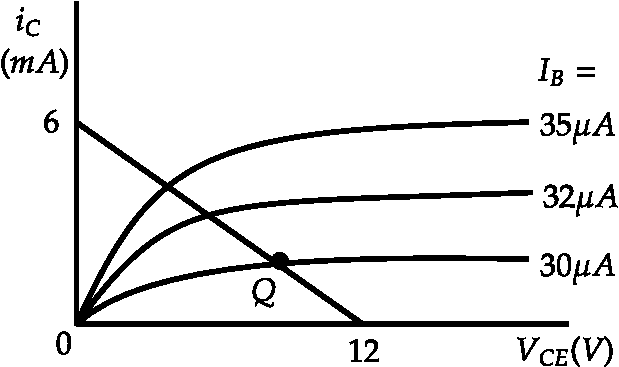
\includegraphics[height=3.3cm,width=5.5cm]{e-17b}
		\end{figure}
		\task[\textbf{C.}] \begin{figure}[H]
			\centering
			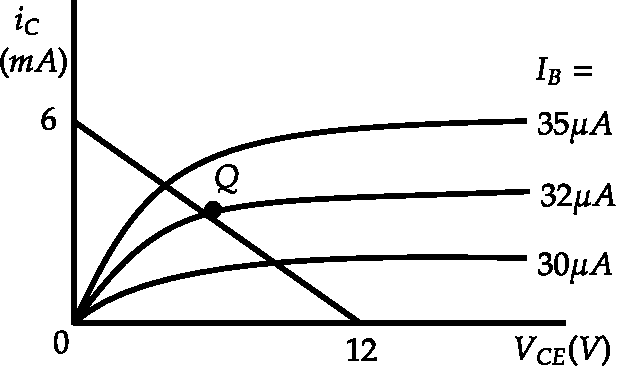
\includegraphics[height=3.3cm,width=5.5cm]{e-17c}
		\end{figure}
		\task[\textbf{D.}] \begin{figure}[H]
			\centering
			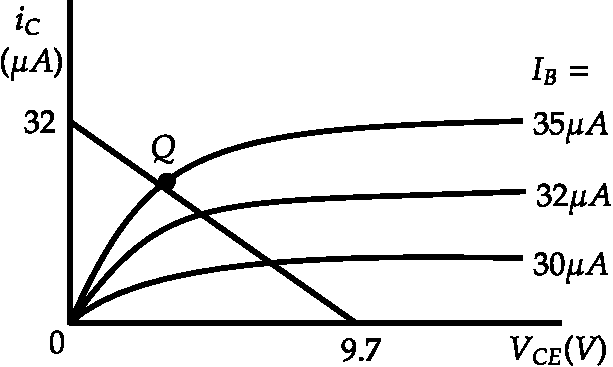
\includegraphics[height=3.3cm,width=5.5cm]{e-17d}
		\end{figure}
	\end{tasks}
	\item The input to a lock-in amplifier has the form $V_{i}(t)=V_{i} \sin \left(\omega t+\theta_{i}\right)$ where $V_{i}, \omega, \theta_{i}$ are the amplitude, frequency and phase of the input signal respectively. This signal is multiplied by a reference signal of the same frequency $\omega$, amplitude $V_{r}$ and phase $\theta_{r}$. If the multiplied signal is fed to a low pass filter of cut-off frequency $\omega$, then the final output signal is
	{	\exyear{NET/JRF(JUNE-2013)}}
	\begin{tasks}(2)
		\task[\textbf{A.}] $\frac{1}{2} V_{i} V_{r} \cos \left(\theta_{i}-\theta_{r}\right)$
		\task[\textbf{B.}] $V_{i} V_{r}\left[\cos \left(\theta_{i}-\theta_{r}\right)-\cos \left(\frac{1}{2} \omega t+\theta_{i}+\theta_{r}\right)\right]$
		\task[\textbf{C.}] $V_{i} V_{r} \sin \left(\theta_{i}-\theta_{r}\right)$
		\task[\textbf{D.}] $V_{i} V_{r}\left[\cos \left(\theta_{i}-\theta_{r}\right)+\cos \left(\frac{1}{2} \omega t+\theta_{i}+\theta_{r}\right)\right]$
	\end{tasks}
	\item An $R C$ network produces a phase-shift of $30^{\circ}$. How many such $R C$ networks should be cascaded together and connected to a Common Emitter amplifier so that the final circuit behaves as an oscillator?
	{	\exyear{NET/JRF(JUNE-2014)}}
	\begin{tasks}(4)
		\task[\textbf{A.}] 6
		\task[\textbf{B.}] 12
		\task[\textbf{C.}] 9
		\task[\textbf{D.}] 3
	\end{tasks}
	\item Consider the circuits shown in figures (a) and (b) below\\
	\begin{figure}[H]
		\centering
		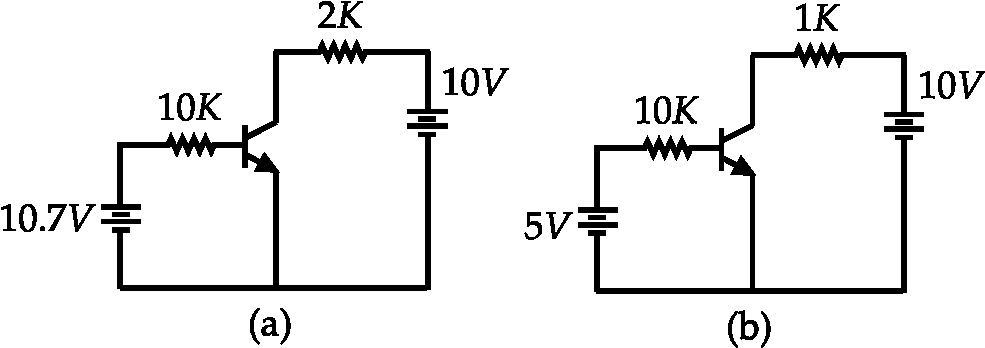
\includegraphics[height=3.2cm,width=9cm]{e-37}
	\end{figure}
	If the transistors in Figures (a) and (b) have current gain $\left(\beta_{d c}\right)$ of 100 and 10 respectively, then they operate in the
	{	\exyear{NET/JRF(JUNE-2015)}}
	\begin{tasks}(1)
		\task[\textbf{A.}] Active region and saturation region respectively
		\task[\textbf{B.}] Saturation region and active region respectively
		\task[\textbf{C.}] Saturation region in both cases
		\task[\textbf{D.}]  Active region in both cases
	\end{tasks}
	\item The $I-V$ characteristics of a device can be expressed as $I=I_{s}\left[\exp \left(\frac{a V}{T}\right)-1\right]$, where $T$ is the temperature and $a$ and $I_{s}$ are constants independent of $T$ and $V$. Which one of the following plots is correct for a fixed applied voltage $V$ ?
	{	\exyear{NET/JRF(DEC-2016)}}
	\begin{tasks}(2)
		\task[\textbf{A.}] \begin{figure}[H]
			\centering
			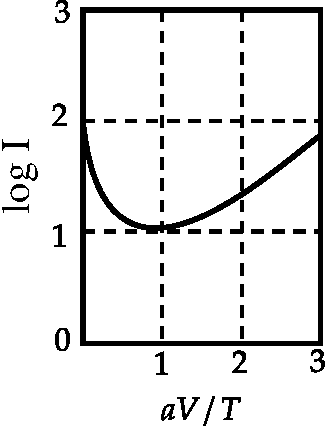
\includegraphics[height=4.5cm,width=3.5cm]{e48a}
		\end{figure}
		\task[\textbf{B.}] \begin{figure}[H]
			\centering
			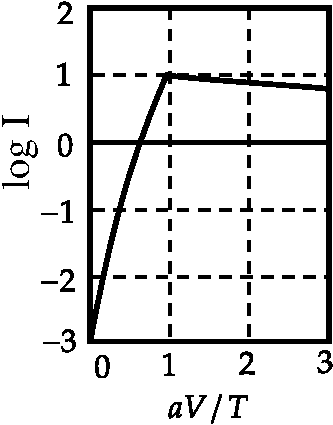
\includegraphics[height=4.5cm,width=3.5cm]{e48b}
		\end{figure}
		\task[\textbf{C.}] \begin{figure}[H]
			\centering
			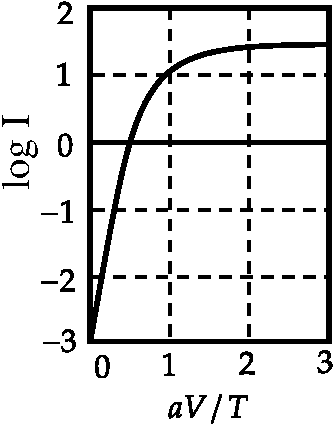
\includegraphics[height=4.5cm,width=3.5cm]{e48c}
		\end{figure}
		\task[\textbf{D.}] \begin{figure}[H]
			\centering
			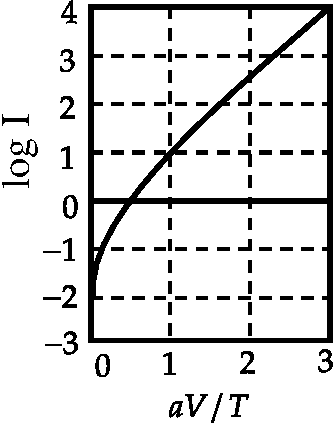
\includegraphics[height=4.5cm,width=3.5cm]{e48d}
		\end{figure}
	\end{tasks}
	\item In the $n$-channel JFET shown in figure below, $V_{i}=-2 V, C=10 p F, V_{D D}=+16 \mathrm{~V}$ and $R_{D}=2 k \Omega$\\
	\begin{figure}[H]
		\centering
		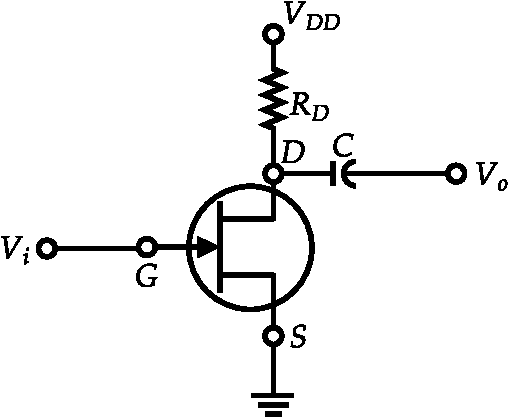
\includegraphics[height=4cm,width=5cm]{e53}
	\end{figure}
	If the drain $D$ - source $S$ saturation current $I_{D S S}$ is $10 m A$ and the pinch-off voltage $V_{P}$ is $-8 V$, then the voltage across points $D$ and $S$ is
	{	\exyear{NET/JRF(JUNE-2017)}}
	\begin{tasks}(4)
		\task[\textbf{A.}] $11.125 \mathrm{~V}$
		\task[\textbf{B.}] $10.375 \mathrm{~V}$
		\task[\textbf{C.}] $5.75 \mathrm{~V}$
		\task[\textbf{D.}] $4.75 \mathrm{~V}$
	\end{tasks}
	\item In the circuit below the voltages $V_{B B}$ and $V_{C C}$ are kept fixed, the voltage measured at $B$ is a constant, but that measured at $A$ fluctuates between a few $\mu V$ to a few $m V$.\\
	From these measurements it may be inferred that the
	{\exyear{NET/JRF(DEC-2017)}}
	\begin{figure}[H]
		\centering
		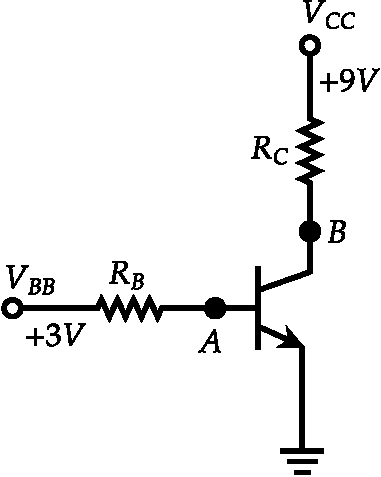
\includegraphics[height=4.5cm,width=4cm]{e63}
	\end{figure}
	\begin{tasks}(2)
		\task[\textbf{A.}] Base is open internally
		\task[\textbf{B.}] Emitter is open internally
		\task[\textbf{C.}] Collector resistor is open
		\task[\textbf{D.}] Base resistor is open
	\end{tasks}
	\item In the following circuit, the value of the common-emitter forward current amplification factor $\beta$ for the transistor is 100 and $V_{B E}$ is $0.7 \mathrm{~V}$.\\
	\begin{figure}[H]
		\centering
		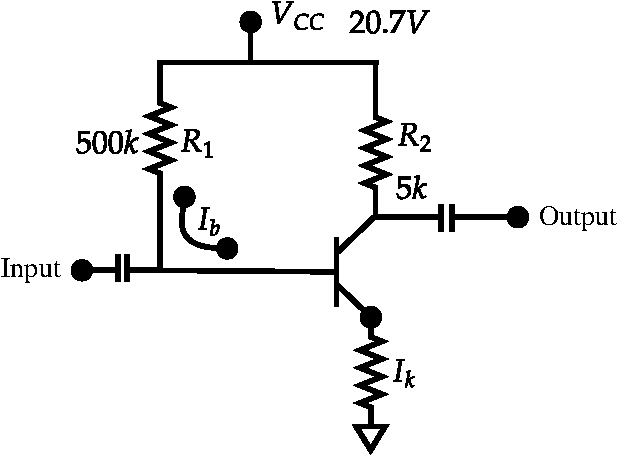
\includegraphics[height=4cm,width=5.5cm]{e68}
	\end{figure}
	The base current $I_{B}$ is
	{	\exyear{NET/JRF(JUNE-2018)}}
	\begin{tasks}(4)
		\task[\textbf{A.}] $40 \mu A$
		\task[\textbf{B.}] $30 \mu A$
		\task[\textbf{C.}] $44 \mu A$
		\task[\textbf{D.}] $33 \mu A$
	\end{tasks}
	\item A sinusoidal signal is an input to the following circuit\\
	\begin{figure}[H]
		\centering
		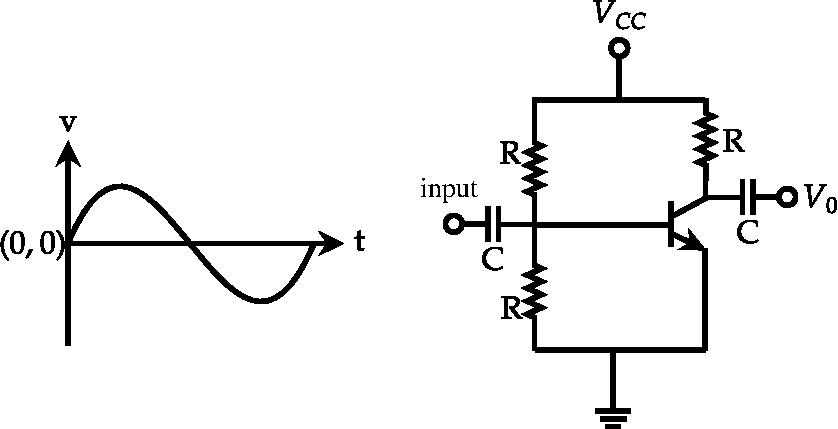
\includegraphics[height=5cm,width=8cm]{e75}
	\end{figure}
	Which of the following graphs best describes the output wave function?
	{	\exyear{NET/JRF(DEC-2018)}}
	\begin{tasks}(2)
		\task[\textbf{A.}] \begin{figure}[H]
			\centering
			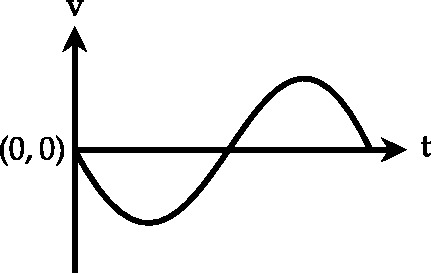
\includegraphics[height=3cm,width=5cm]{e75a}
		\end{figure}
		\task[\textbf{B.}] \begin{figure}[H]
			\centering
			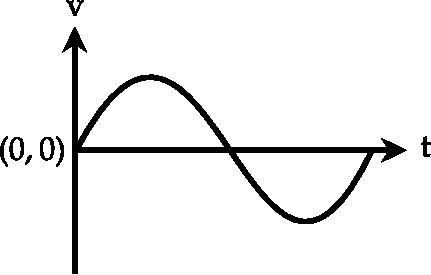
\includegraphics[height=3cm,width=5cm]{e75b}
		\end{figure}
		\task[\textbf{C.}] \begin{figure}[H]
			\centering
			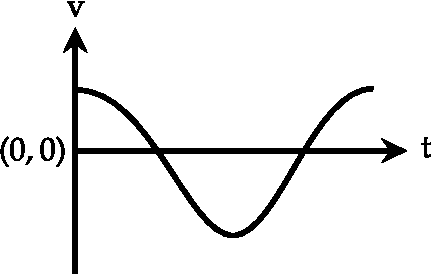
\includegraphics[height=3cm,width=5cm]{e75c}
		\end{figure}
		\task[\textbf{D.}] \begin{figure}[H]
			\centering
			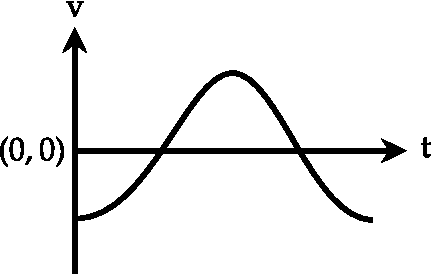
\includegraphics[height=3cm,width=5cm]{e76d}
		\end{figure}
	\end{tasks}
	\item An $npn$ -transistor is connected in a voltage divider configuration as shown in the figure below\\
	\begin{figure}[H]
		\centering
		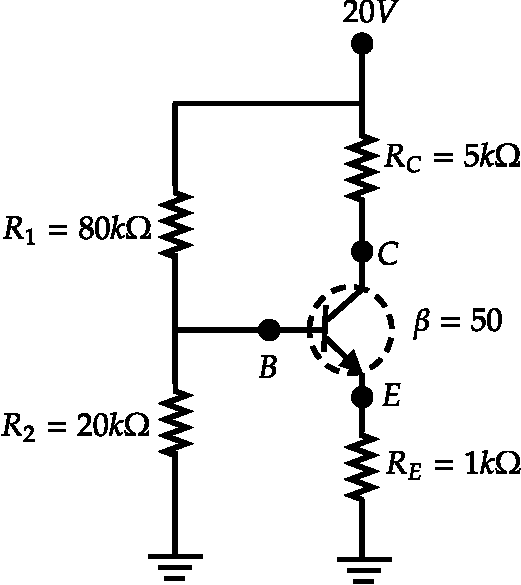
\includegraphics[height=6cm,width=5.5cm]{e-2}
	\end{figure}
	If the resistor $R_{2}$ is disconnected, the voltages $V_{B}$ at the base and $V_{C}$ at the collector change as follows.
	{	\exyear{NET/JRF(JUNE-2019)}}
	\begin{tasks}(2)
		\task[\textbf{A.}]  Both $V_{B}$ and $V_{C}$ increase
		\task[\textbf{B.}] Both $V_{B}$ and $V_{C}$ decrease
		\task[\textbf{C.}]  $V_{B}$ decreases, but $V_{C}$ increases
		\task[\textbf{D.}] $V_{B}$ increases, but $V_{C}$ decreases
	\end{tasks}
	\item In a collector feedback circuit shown in the figure below, the base emitter voltage $V_{B E}=0.7 V$ and current gain $\beta=\frac{I_{C}}{I_{B}}=100$ for the transistor\\
	\begin{figure}[H]
		\centering
		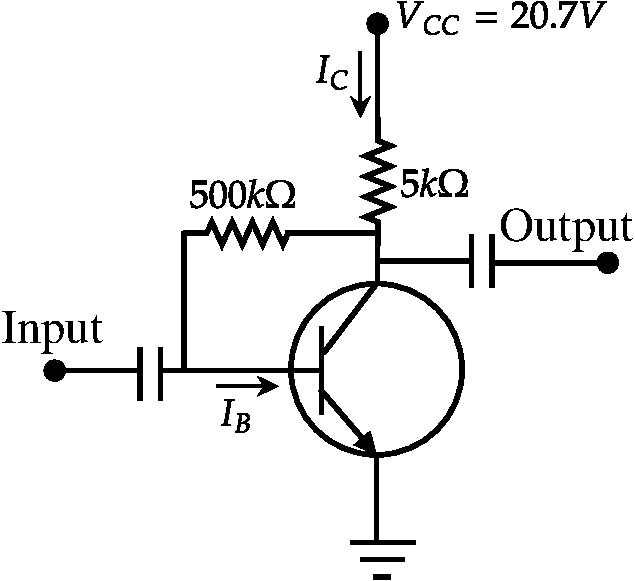
\includegraphics[height=5.5cm,width=6cm]{e-3}
	\end{figure}
	The value of the base current $I_{B}$ is
	{	\exyear{NET/JRF(DEC-2019)}}
	\begin{tasks}(4)
		\task[\textbf{A.}] $20 \mu \mathrm{A}$
		\task[\textbf{B.}]  $40 \mu \mathrm{A}$
		\task[\textbf{C.}] $10 \mu \mathrm{A}$
		\task[\textbf{D.}] $100 \mu \mathrm{A}$
	\end{tasks}
\end{enumerate}
 \colorlet{ocre1}{ocre!70!}
\colorlet{ocrel}{ocre!30!}
\setlength\arrayrulewidth{1pt}
\begin{table}[H]
	\centering
	\arrayrulecolor{ocre}
	\begin{tabular}{|p{1.5cm}|p{1.5cm}||p{1.5cm}|p{1.5cm}|}
		\hline
		\multicolumn{4}{|c|}{\textbf{Answer key}}\\\hline\hline
		\rowcolor{ocrel}Q.No.&Answer&Q.No.&Answer\\\hline
		1&\textbf{A} &2&\textbf{B}\\\hline 
		3&\textbf{A} &4&\textbf{A} \\\hline
		5&\textbf{B} &6&\textbf{D} \\\hline
		7&\textbf{D}&8&\textbf{D}\\\hline
		9&\textbf{D}&10&\textbf{A}\\\hline
		11&\textbf{D} &12&\textbf{A}\\\hline
		
	\end{tabular}
\end{table}
\newpage
\begin{abox}
	Practice set 2 
	\end{abox}
\begin{enumerate}
	\begin{minipage}{\textwidth}
		\item  A transistor is $\cdots$ a operated device
	\end{minipage}
	\begin{tasks}(2)
		\task[\textbf{A.}] current
		\task[\textbf{B.}] voltage
		\task[\textbf{C.}]both voltage and current
		\task[\textbf{D.}]none of the above
	\end{tasks}
\begin{minipage}{\textwidth}
	\item In a transistor, the base current is about ………….. of emitter current
\end{minipage}
\begin{tasks}(2)
	\task[\textbf{A.}] $25 \%$
	\task[\textbf{B.}] $20 \%$
	\task[\textbf{C.}] $35 \%$
	\task[\textbf{D.}]$4.5 \%$ 
\end{tasks}
\begin{minipage}{\textwidth}
	\item The element that has the biggest size in a transistor is ………………..
\end{minipage}
\begin{tasks}(2)
	\task[\textbf{A.}] collector
	\task[\textbf{B.}] collector base junction
	\task[\textbf{C.}]base
	\task[\textbf{D.}]emitter
\end{tasks}
	 \begin{minipage}{\textwidth}
		\item An $R C$ network produces a phase-shift of $30^{\circ} .$ How many such $R C$ networks should be cascaded together and connected to a Common Emitter amplifier so that the final circuit behaves as an oscillator?
	\end{minipage}
	\begin{tasks}(2)
		\task[\textbf{A.}] 6
		\task[\textbf{B.}] 12
		\task[\textbf{C.}]9
		\task[\textbf{D.}]3
	\end{tasks}
\begin{minipage}{\textwidth}
	\item In the circuit below the voltages $V_{B B}$ and $V_{C C}$ are kept fixed, the voltage measured at $B$ is a constant, but that measured at $A$ fluctuates between a few $\mu V$ to a few $m V$.
	From these measurements it may be inferred that the\\
\begin{figure}[H]
	\centering
	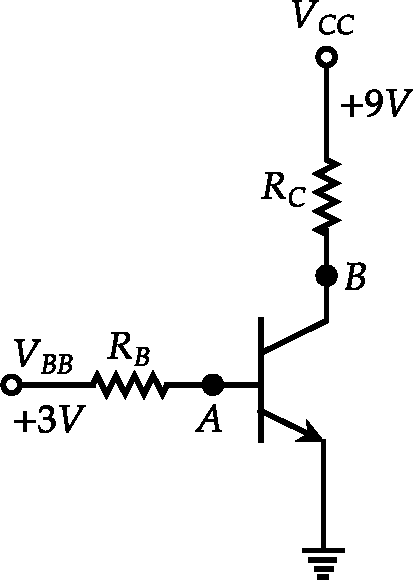
\includegraphics[height=5cm,width=4cm]{diagram-20211208(1)-crop}
\end{figure}
\end{minipage}
\begin{tasks}(2)
	\task[\textbf{A.}]base is open internally 
	\task[\textbf{B.}] emitter is open internally
	\task[\textbf{C.}]collector resistor is open
	\task[\textbf{D.}]base resistor is open
\end{tasks}
\begin{minipage}{\textwidth}
	\item A sinusoidal signal is an input to the following circuit\\
\begin{figure}[H]
	\centering
	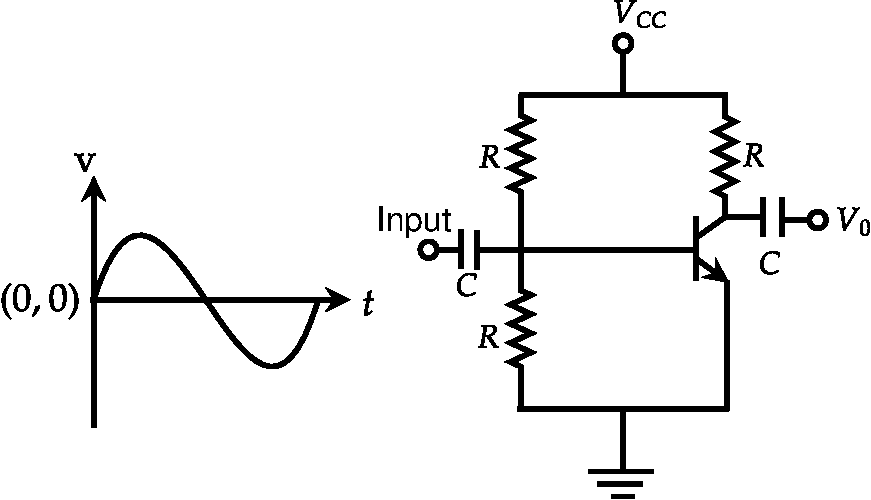
\includegraphics[height=4cm,width=8cm]{diagram-20211109(3)-crop}
\end{figure}
	Which of the following graphs best describes the output wave function?
\end{minipage}
\begin{tasks}(2)
	\task[\textbf{A.}]\begin{figure}[H]
		\centering
		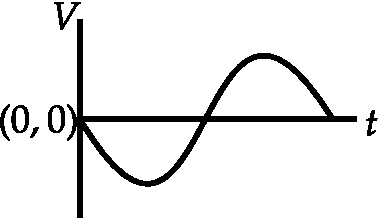
\includegraphics[height=2.5cm,width=4cm]{diagram-20211109(4)-crop}
	\end{figure}
	\task[\textbf{B.}] \begin{figure}[H]
		\centering
		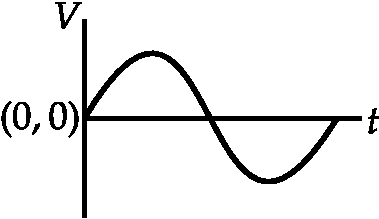
\includegraphics[height=2.5cm,width=4cm]{diagram-20211109(5)-crop}
	\end{figure}
	\task[\textbf{C.}]\begin{figure}[H]
		\centering
		\includegraphics[height=2.5cm,width=4cm]{diagram-20211109(6)-crop}
	\end{figure}
	\task[\textbf{D.}]\begin{figure}[H]
		\centering
		\includegraphics[height=2.5cm,width=4cm]{diagram-20211109(7)-crop}
	\end{figure}
\end{tasks}
\begin{minipage}{\textwidth}
	\item  The power gain in a transistor connected in ........
	arrangement is the highest
\end{minipage}
\begin{tasks}(1)
	\task[\textbf{A.}]common emitter 
	\task[\textbf{B.}] common base
	\task[\textbf{C.}]common collector
	\task[\textbf{D.}]	none of the above
\end{tasks}
\begin{minipage}{\textwidth}
	\item  In a transistor, signal is transferred from a ................
	circuit
	    
\end{minipage}
\begin{tasks}(1)
	\task[\textbf{A.}] high resistance to low resistance
	\task[\textbf{B.}] low resistance to high resistance
	\task[\textbf{C.}]high resistance to high resistance
	\task[\textbf{D.}]low resistance to low resistance
\end{tasks}
\begin{minipage}{\textwidth}
	\item  What is the region on the output characteristics for $\mathrm{V}_{\mathrm{CE}}<\mathrm{V}_{\mathrm{CE}_{\mathrm{sat}}}$ called?
\end{minipage}
\begin{tasks}(1)
	\task[\textbf{A.}]  Active region
	\task[\textbf{B.}] Cutoff region
	\task[\textbf{C.}]Saturation region
	\task[\textbf{D.}]Active \& Cutoff region
\end{tasks}
\begin{minipage}{\textwidth}
	\item 1. Which of the following is the correct relationship between base and emitter current of a BJT?
\end{minipage}
\begin{tasks}(1)
	\task[\textbf{A.}]$\mathrm{I}_{\mathrm{B}}=\beta \mathrm{I}_{\mathrm{E}}$ 
	\task[\textbf{B.}] $\mathrm{I}_{\mathrm{B}}=\mathrm{I}_{\mathrm{E}}$
	\task[\textbf{C.}]$\mathrm{I}_{\mathrm{B}}=(\beta+1) \mathrm{I}_{\mathrm{E}}$
	\task[\textbf{D.}]$\mathrm{I}_{\mathrm{E}}=(\beta+1) \mathrm{I}_{\mathrm{B}}$
\end{tasks}
\begin{minipage}{\textwidth}
	\item 1. For a BJT, for common base configuration the input characteristics are represented by a plot between which of the following parameters?
\end{minipage}
\begin{tasks}(1)
	\task[\textbf{A.}] $V_{B E}$ and $I_{E}$
	\task[\textbf{B.}] $V_{B E}$ and $I_{B}$
	\task[\textbf{C.}]$\mathrm{V}_{\mathrm{CE}}$ and $\mathrm{I}_{\mathrm{C}}$
	\task[\textbf{D.}] $\mathrm{V}_{\mathrm{CC}}$ and $\mathrm{I}_{\mathrm{C}}$
\end{tasks}
\begin{minipage}{\textwidth}
	\item In a BJT, if the collector-base junction is reverse-biased and the base-emitter junction is forward-biased, which region is the BJT operating in?
\end{minipage}
\begin{tasks}(1)
	\task[\textbf{A.}] Saturation region
	\task[\textbf{B.}]  Active region
	\task[\textbf{C.}] Cutoff region
	\task[\textbf{D.}]Reverse active region
\end{tasks}
\begin{minipage}{\textwidth}
	\item In amplifier circuit, biasing of transistor is necessary to
\end{minipage}
\begin{tasks}(1)
	\task[\textbf{A.}] Fix the value of current amplification
	\task[\textbf{B.}]Establish suitable D.C working conditions 
	\task[\textbf{C.}]Ensure that transistor is saturated
	\task[\textbf{D.}]transistor
\end{tasks}
\begin{minipage}{\textwidth}
	\item  An amplifier has a power gain of 100 . Its db gain is
\end{minipage}
\begin{tasks}(1)
	\task[\textbf{A.}] $10 \mathrm{db}$
	\task[\textbf{B.}] $20 \mathrm{db}$
	\task[\textbf{C.}]$40 \mathrm{db}$
	\task[\textbf{D.}] None of the above
\end{tasks}
\begin{minipage}{\textwidth}
	\item The purpose of emitter capacitor (i.e. capacitor across $R E$ ) is to
\end{minipage}
\begin{tasks}(1)
	\task[\textbf{A.}]  Avoid voltage gain drop
	\task[\textbf{B.}] Forward bias the emitter
	\task[\textbf{C.}]Reduce noise in the amplifier
	\task[\textbf{D.}]None of the above
\end{tasks}
\begin{minipage}{\textwidth}
	\item  A transistor converts
\end{minipage}
\begin{tasks}(1)
	\task[\textbf{A.}]d.c. power into a.c. power 
	\task[\textbf{B.}] a.c. power into d.c. power
	\task[\textbf{C.}]high resistance into low resistance
	\task[\textbf{D.}]none of the above
\end{tasks}
\end{enumerate}
\colorlet{ocre1}{ocre!70!}
\colorlet{ocrel}{ocre!30!}
\setlength\arrayrulewidth{1pt}
\begin{table}[H]
	\centering
	\arrayrulecolor{ocre}
	
	\begin{tabular}{|p{1.5cm}|p{1.5cm}||p{1.5cm}|p{1.5cm}|}
		\hline
		\multicolumn{4}{|c|}{\textbf{Answer key}}\\\hline\hline
		\rowcolor{ocrel}Q.No.&Answer&Q.No.&Answer\\\hline
		1&\textbf{a}&2&\textbf{d}\\\hline
		3&\textbf{a}&4&\textbf{a}\\\hline
		5&\textbf{d}&6&\textbf{a}\\\hline
		7&\textbf{a}&8&\textbf{b}\\\hline
		9&\textbf{c}&10&\textbf{c}\\\hline
		11&\textbf{a}&12&\textbf{b}\\\hline
		13&\textbf{a}&14&\textbf{b}\\\hline
		15&\textbf{a}&&\\\hline
	\end{tabular}
\end{table}
\newpage
\begin{abox}
	Practice set 3
	\end{abox}
\begin{enumerate}
		\begin{minipage}{\textwidth}
		\item A transistor-oscillator using a resonant circuit with an inductor $\mathrm{L}$ ( of negligible resistance ) and a capacitor $\mathrm{C}$ in series produce oscillations of frequency $\mathrm{f}$. If $\mathrm{L}$ is doubled and $\mathrm{C}$ is changed to $4 \mathrm{C}$, the frequency will be
	\end{minipage}
	\begin{answer}
		$$f=\frac{1}{2\pi}\frac{1}{\sqrt{LC}}$$
		$$f^{\prime}=\frac{1}{2\pi}\frac{1}{\sqrt{2L4C}}$$
		$$f^{\prime}=\frac{f}{2\sqrt{2}}$$
	\end{answer}
	\begin{minipage}{\textwidth}
	\item The $\beta$ of a transistor is 50 . The input resistance of the transistor when used in the common emitter configuration is $2 \mathrm{k} \Omega$. The peak value of the collector AC current for an AC input voltage of $0.02 \mathrm{~V}$ peak is
\end{minipage}
\begin{answer}
	$$R_i=2k\Omega \quad \beta=50 \quad V_i=0.02V$$
	$$i_{b}=\frac{0.02}{2\times 10^3}=10^{-5}A$$
	$$\beta=\frac{I_C}{I_B}$$
	$$I_C=I_B\times \beta $$
	$$=50\times 10^{_5}=500\mu A$$
\end{answer}
	\begin{minipage}{\textwidth}
	\item In CE transistor amplifier, the audio signal voltage across the collector resistance of $2 \mathrm{k} \Omega$ is $2 \mathrm{~V}$. If the base resistance is $1 \mathrm{k} \Omega$ and the current amplification of the transistor is 100 , the input signal voltage is
\end{minipage}
\begin{answer}
	\begin{align*}
	V_0=2V \quad R_C&=2\times 10^3\Omega \quad R_B=1\times 10^3\Omega \quad v_i=?\\
	V_0&=I_CR_C=2\\
	I_C&=\frac{2}{R_C}=\frac{2}{2\times 10^3}=10^{-3}\\
	\beta&=\frac{I_C}{I_B}=100\\
	I_B&=\frac{I_C}{100}=\frac{10^{-3}}{100}=10^{-5}\\
	V_i&=R_BI_B=1\times 10^3 \times 10^{-5}=10mV
	\end{align*}
\end{answer}
		\begin{minipage}{\textwidth}
		\item In circuit shown, assume that the transistor is in active region. It has a large $\beta$ and its base emitter voltage is $0.7$ volts. The value of $\mathrm{I}_{\mathrm{C}}$ is
		\begin{figure}[H]
			\centering
			\includegraphics[height=5cm,width=4cm]{diagram-20211109(19)-crop}
		\end{figure}
	\end{minipage}
	\begin{answer}
		$$\beta=\frac{I_C}{I_B}$$
		$$I_B=\frac{I_C}{\beta}$$
		When $\beta$ is large \\
		$$I_B\approx 0$$
		Consider the loop containing base emitter junction.Then 
		$$V_B=V_{BE}+I_ER_E$$
		$$V_B=\frac{15}{10+5}\times 5$$
		$$V_B=5V$$
		$$I_E=\frac{V_B-V_{BE}}{R_E}$$
		$$I_E=\frac{5-0.7}{430}$$
		$$=10mA$$
	\end{answer}
		\begin{minipage}{\textwidth}
		\item Consider the circuits shown in figures (a) and (b) below
		\begin{figure}[H]
			\centering
			\includegraphics[height=4cm,width=10cm]{diagram-20211108(13)-crop}
		\end{figure}
		If the transistors in Figures (a) and (b) have current gain $\left(\beta_{d c}\right)$ of 100 and 10 respectively, then they operate in the\\
	\end{minipage}
	\begin{answer}
	In both case input section is F.B.\\
		For figure (a) $I_{B}=\frac{10.7-0.7}{10}=1 \mathrm{~mA} \Rightarrow I_{C}=B I_{B}=100 \mathrm{~mA}$\\
		Thus $V_{C B}=V_{C}-V_{B}=(10-2 \times 100)-0.7=-v e$\\
		$\Rightarrow \quad$ output section is F.B.\\
		since both section are F.B. so it is in saturation region.\\
		For Figure (b) $I_{B}=\frac{5-0.7}{10}=0.43 \mathrm{~mA} \Rightarrow I_{C}=B I_{B}=4.3 \mathrm{~mA}$\\
		Thus $\left.V_{C B}=V_{C}-V_{B}=(10-4.3)-0.7\right)=+v e$\\
		$\Rightarrow \quad$ out put section is R.B.\\
		Thus it is in active region
\end{answer}
	\begin{minipage}{\textwidth}
	\item  It is desired to set the operating point at $2 \mathrm{~V}, 1 \mathrm{~mA}$ by biasing a silicon transistor with collector feedback resistor RB. If $\beta=100$, find the value of $R_B$
	\begin{figure}[H]
		\centering
		\includegraphics[height=6cm,width=4.5cm]{diagram-20211109(10)-crop}
	\end{figure}
\end{minipage}
\begin{answer}
\begin{align*}
I_C=1mA \quad \beta=100 \quad V_{CE}=2V\\
\beta=\frac{I_C}{I_B}\\
I_B=\frac{I_C}{\beta}=\frac{1mA}{100=10}=10\mu A\\
V_{CE}=V_{BE}+V_{CB}\\
2=0.7V+V_{CB}\\
V_{CB}=2-0.7=1.3V\\
R_B=\frac{V_{CB}}{I_B}=\frac{1.3V}{10 \mu A}=130K\Omega
\end{align*}	
\end{answer}
	\begin{minipage}{\textwidth}
	\item Calculate the emitter current in the voltage divider circuit shown in Figure?
	\begin{figure}[H]
		\centering
		\includegraphics[height=6cm,width=7cm]{diagram-20211109(11)-crop}
	\end{figure}
	Also find the value of $V_{CE} $ and collector potential $V_C$
\end{minipage}
\begin{answer}
\begin{align*}
V_2=\frac{V_{CC}}{R_1+R_2}\times R_2\\
=\frac{20}{10+10}\times 10=10V\\
V_2=V_{BE}+I_ER_E\\
V_2=I_ER_E\\
I_E=\frac{V_2}{R_E}=\frac{10}{5k\Omega}=2mA\\
I_E\approx I_C\\
V_{CC}=I_CR_C+V_{CE}+I_ER_E\\
V_{CC}=I_ER_C+V_{CE}+I_ER_E\\
V_{CC}=V_{CE}+I_E(R_C+R_E)\\
V_{CE}=V_{CC}-I_E(R_C+R_E)\\
V_{CE}=20-2\times 10^{-3}(1+5)\times 10^3\\
=20-12=8V\\
V_C=V_{CC}-I_CR_C\\
=20-2\times 10^{-3}\times 1 \times 10^3\\
20-2=18V
\end{align*}	
\end{answer}
	\begin{minipage}{\textwidth}
	\item Refer to this figure. The value of $V_{C E}$   is?
	\begin{figure}[H]
		\centering
		\includegraphics[height=5cm,width=7cm]{diagram-20211109(12)-crop}
	\end{figure}
\end{minipage}
\begin{answer}
	Consider the loop containing base resisitor and battery 5V.
	\begin{align*}
	V_2=I_BR_B+V_{BE}\\
	I_BR_B=V_2-V_{BE}\\
	5-0.7=4.3V\\
	I_B=\frac{4.3}{5k\Omega}=0.86mA\\
	I_C=I_B\times \beta=0.86\times 25=21.5mA\\
	V_{CC}=I_CR_C+V_{CE}\\
	V_{CE}=V_{CC}-I_CR_C\\
	=20-21.5\times 470 \times 10^{-3}=9.9V
	\end{align*}
\end{answer}
	\begin{minipage}{\textwidth}
	\item A transistor having $\alpha=0.99$ and $\mathrm{V}_{\mathrm{BE}}=0.7$ volts, in the circuit shown, then the value of the collector current will be.............
	\begin{figure}[H]
		\centering
		\includegraphics[height=6cm,width=4cm]{diagram-20211109(9)-crop}
	\end{figure}
\end{minipage}
\begin{answer}
	Consider the loop containing collector resisitor $R_C=1k\Omega$
\begin{align*}
V_{CC}&=(I_B+I_C)\times 10^3+I_C\times 10^3+V_{CE}+(I_B+I_C)\times 10^3\\
I_E&=I_B+I_C\\
12&=2I_B+2I_C+I_C+0.2V\\
11.8&=3I_C+2I_B\\
\text{Suppose the transistor is at saturation then }& V_{CE(sat)}=0.2V \quad and \quad V_{BE(sat)}=0.8V\\
\text{Consider the loop containing base resisitor} R_B&=10k\Omega\\
V_{CC}&=(I_B+I_C)1\times 10^3+I_B\times 10\times 10^3+V_{CE(sat)}+(I_B+I_C)\times 10^3\\
12&=12I_B+2I_C+0.8\\
11.2&=12I_B+2I_C\\
11.8&=3I_C+2I_B\\
\text{From these two equations we will get }\\
I_C&=3.725mA
\end{align*}	
\end{answer}
	\begin{minipage}{\textwidth}
	\item The input signal given to a a CE amplifier having a voltage gain of 150 is $\mathrm{V}_{\mathrm{i}}=2 \cos \left(15 \mathrm{t}+\frac{\pi}{3}\right)$. The corresponding output signal will be
\end{minipage}
\begin{answer}
$$V_i=2\cos(15t+\frac{\pi}{3})$$
voltage gain $A_v=\frac{V_0}{V_i}$
$$V_0=A_v\times V_i$$
$$=150\times 2 \cos (15t+\frac{\pi}{3})	$$
$$=300\cos (15t+\frac{\pi}{3})$$
Input and output are out of phase in CE configuration.So an additional $\pi$ will come in output voltage\\
$$V_0=300\cos (15t+\frac{\pi}{3}+\pi)$$
$$=300\cos(15t+\frac{4\pi}{3})$$
\end{answer}	
\end{enumerate}
\newpage
